%%
%% 修士論文
%%
%% USE 機能的に等しい
%% not 外的振る舞いが等しい
%%
%% USE 大規模言語モデル
%% not LLM
%%
%% USE 低下させる
%% not 下げる
%%

%%%%%%%%%%%%%%%%%%%%%%%%%%%%%%%%%%%%%%%%%%%%%%%%%%%%%%%%%%%%%%%%

%%
%% 利用するコマンドの準備
%%

%% 必須パッケージ
\documentclass[11pt]{jreport}
\usepackage{wuse_thesis}
\usepackage{indentfirst}

%% 追加パッケージ
%\usepackage{graphicx}
\usepackage{comment}
\usepackage[dvipdfmx]{graphicx}
\usepackage{url}

\usepackage{latexsym}

\usepackage{cite}
\usepackage{amsmath,amssymb,amsfonts}
\usepackage{algorithmic}
\usepackage{textcomp}
\usepackage{xcolor}
\usepackage{listings}
\def\BibTeX{{\rm B\kern-.05em{\sc i\kern-.025em b}\kern-.08em
    T\kern-.1667em\lower.7ex\hbox{E}\kern-.125emX}}


\newcommand{\todo}[1]{\colorbox{yellow}{{\bf TODO}:}{\color{red} {\textbf{[#1]}}}}
\newcommand{\memo}[1]{\colorbox{yellow}{{\bf MEMO}:}{\color{red} {\textbf{[#1]}}}}


\lstset{
basicstyle=\small\ttfamily,
abovecaptionskip=0pt,
captionpos=b,
frame=tb,
framexleftmargin=2em,
numbers=left,
numberstyle={\scriptsize},
xleftmargin=\parindent
}

%ListingのキャプションがFigureになってしまうのをListingに直すコマンド
\usepackage{caption}
\makeatletter
\let\MYcaption\@makecaption
\makeatother
\usepackage{caption}
\makeatletter
\let\@makecaption\MYcaption
\makeatother

\def\Underline{\setbox0\hbox\bgroup\let\\\endUnderline}
\def\endUnderline{\vphantom{y}\egroup\smash{\underline{\box0}}\\}
\def\|{\verb|}
%


%%%%%%%%%%%%%%%%%%%%%%%%%%%%%%%%%%%%%%%%%%%%%%%%%%%%%%%%%%%%%%%%

%%
%% 主に表紙を作成するための情報
%%

%% タイトル(修論の場合は英語表記も指定)
\title{マイクロベンチマーク共有サービスを活用した\\高速化のための自動リファクタリング}
\etitle{Automatic refactoring for faster execution\\using micro-benchmark sharing services}

%% 著者名(修論の場合は英語表記も指定)
\author{大森 楓己}
\eauthor{Fuki Omori}

%% 修士論文(M2用)
\master

%% 学科・クラスタ
\department{システム工}

%% 学生番号
\studentid{S2320027}

%% 卒業年度
\gyear{2024}

%% 論文提出日(修士の場合は月まで)
\date{2025年2月}
\edate{February 2025}


%%%%%%%%%%%%%%%%%%%%%%%%%%%%%%%%%%%%%%%%%%%%%%%%%%%%%%%%%%%%%%%%

%%
%% 表紙・概要・目次
%%

\begin{document}

%% 表紙
\maketitle

%% 概要
\begin{abstract}
%% 開発者の習得方法・マイクロベンチマーク共有サービス
マイクロベンチマーク共有サービスは,JavaScript開発者が高速・可換な実装を学び,他の開発者と共有できるWebサービスである.
開発者は,サービス上で機能的に等しいプログラムの実行速度を測定・比較することで,より高速な実装を学習できる.
さらに,比較したプログラムセット(マイクロベンチマーク)は保存され,すべてのユーザに公開される.
そのため,開発者は他者のマイクロベンチマークから未知の実装を学習できる.

% マイクロベンチマークが未だ利用されていないこと・研究内容
開発者は膨大なマイクロベンチマークから未知の実装を学習できるものの,自動高速化手法への活用は著者の知る限り提案されていない.
本研究では,マイクロベンチマーク共有サービスから収集したプログラムセット内の各実装に対して,実行時間を測定し,統計的な処理に基づいて低速な実装と高速な実装に分類する.
そして,本研究独自の手法による実装間の機能的な等価性の検証および前処理を行うことで,自動リファクタリングモデルの学習に利用できる大規模な実装対データセットを作成する.
さらに,実装対データセットを用いて代表的な2種の自動修正手法(パターンマッチ,深層学習)を用いた高速化のための自動リファクタリングモデルを作成する.
そして,既存の大規模言語モデルや開発者の修正と比較することで,マイクロベンチマークを学習した自動リファクタリングモデルの修正性能を調査する.

% 貢献っぽいこと
本研究により,高速化のための自動リファクタリングモデルの作成に利用できる39,009件の実装対データセットを作成したとともに,作成した実装対データセットを学習させた自動リファクタリングモデルの高速化性能を明らかにした.
\end{abstract}

%% 目次
\tableofcontents

%% 図目次
%\listoffigures

%% 表目次
%\listoftables

\newpage
\pagenumbering{arabic}


%%%%%%%%%%%%%%%%%%%%%%%%%%%%%%%%%%%%%%%%%%%%%%%%%%%%%%%%%%%%%%%%

%%
%% 1 はじめに
%%

\chapter{はじめに}\label{chapter:intro}


%% 実装が複数あること・品質が異なること
高水準言語では,用いる構文やライブラリ,アルゴリズム等により,しばしば単一の機能要件に対して複数の実装が考えられる.
しかし,実現する機能が等しい実装であっても,性能効率性や保守性等の非機能要件への影響は各々異なる.
そのため,実装によってはソフトウェア品質を低下させる場合がある.
特に,些細な品質低下は開発者に見逃され,プロダクトに蓄積することでソフトウェア品質を漸次的に低下させ続ける恐れがある.

%% 品質の向上・リファクタリング
ソフトウェア品質の低下を防ぐため,しばしば開発者は既存の実装を機能的に等しく,より品質の高い実装に書き換えることで品質低下を防ぐ.
この書き換えはリファクタリングと呼ばれ,性能効率性や保守性等のさまざまな品質を高めるために行われる.
例として,Webアプリケーション開発者はリファクタリングによってプログラム処理を高速化する\cite{Selakovic_2016}.
Webアプリケーションの高速化はプロダクトの性能効率性を高めるだけでなく,Interaction to Next Paint\footnote{\url{https://web.dev/articles/inp/}}の向上による検索エンジン最適化にもつながる重要なタスクの1つである.

%% リファクタリング一般の支援状況
現在までに,リファクタリングを支援する手法は多数提案されている.
例として,ESLint\footnote{\url{https://eslint.org/}}やBiome\footnote{\url{https://biomejs.dev/}}等の静的解析ツールは命名規則違反や文法上の問題を自動検出・修正することで,プログラムの可読性を効率的に維持・向上する.

%% 高速化リファクタリングの難しさ
可読性のためのリファクタリングが静的解析ツールによって効率化されている一方で,プログラムの高速化については,ベンチマークテストが速度低下の検出・原因箇所の特定に用いられるものの,多くの修正は未だ開発者に委ねられている\todo{引用}.
特に,JavaScriptに代表される動的型付け言語は単一の変数に異なる型のオブジェクトを再代入できるため,修正箇所の特定には文脈に基づく高度な技術的判断を要する.
さらに,多くの動的型付け言語はインタプリタ言語であり,コンパイラ言語に比べて低速である.そのため,動的型付け言語の高速化に対する支援不足は非常に重大な課題であると考えられる.
本研究では,マイクロベンチマーク共有サービスを活用して自動リファクタリングモデルを作成することで,プログラムの高速化の支援を目指す.

%% 開発者の習得方法・マイクロベンチマーク共有サービス
マイクロベンチマーク共有サービスは,JavaScript開発者が高速・可換な実装を学び,他の開発者と共有できるWebサービスである.
開発者は,サービス上で機能的に等しいプログラムの実行速度を測定・比較することで,より高速な実装を学習できる.
さらに,比較したプログラムセット(マイクロベンチマーク)は保存され,すべてのユーザに公開される.
そのため,開発者は他者のマイクロベンチマークから未知の実装を学習できる.

% マイクロベンチマークが未だ利用されていないこと・研究内容
開発者は膨大なマイクロベンチマークから未知の実装を学習できるものの,自動高速化手法への活用は著者の知る限り提案されていない.
本研究では,マイクロベンチマーク共有サービスから収集したプログラムセット内の各実装に対して,実行時間を測定し,統計的な処理に基づいて低速な実装と高速な実装に分類する.
そして,本研究独自の手法による実装間の機能的な等価性の検証および前処理を行うことで,自動リファクタリングモデルの学習に利用できる大規模な実装対データセットを作成する.
さらに,実装対データセットを用いて代表的な2種の自動修正手法(パターンマッチ,深層学習)を用いた高速化のための自動リファクタリングモデルを作成する.
そして,既存の大規模言語モデルや開発者の修正と比較することで,マイクロベンチマークを学習した自動リファクタリングモデルの修正性能を調査する.

% 貢献っぽいこと
本研究により,高速化のための自動リファクタリングモデルの作成に利用できる39,009件の実装対データセットを作成したとともに,作成した実装対データセットを学習させた自動リファクタリングモデルの高速化性能を明らかにした.

%% 章立て
続く\ref{chapter:related-work}章では,本研究の関連研究について述べる.\ref{chapter:dataset}章および\ref{chapter:model}章では,本研究の提案手法について述べ,\ref{chapter:eval-1}章では評価手法について述べる.そして\ref{chapter:threats}章で本研究の妥当性の脅威を述べた後,\ref{chapter:conc}章で総括する.


%%%%%%%%%%%%%%%%%%%%%%%%%%%%%%%%%%%%%%%%%%%%%%%%%%%%%%%%%%%%%%%%

%%
%% 2 関連研究
%%

\chapter{関連研究}\label{chapter:related-work}


%%%%%%%%%%%%%%%%%%%%%%%%%%%%%%%%%%%%%%%%%%%%%%%%%%%%%%%%%%%%%%%%

%%
%% 2.1 マイクロベンチマーク共有サービス
%%

\section{マイクロベンチマーク共有サービス}


%%%%%%%%%%%%%%%%%%%%%%%%%%%%%%%%%%%%%%%%%%%%%%%%%%%%%%%%%%%%%%%%

%%
%% 2.1.1 マイクロベンチマーク
%%

\subsection{マイクロベンチマーク}


マイクロベンチマークは,非常に小さなプログラム断片を比較されるプログラムセットである.
Listing~\ref{ex-microbenchmark-setup}およびListing~\ref{ex-microbenchmark-test-1},Listing~\ref{ex-microbenchmark-test-2}にマイクロベンチマークの例\todo{引用}を示す.

\begin{figure}[t]
\captionsetup{name=Listing}
\hspace{0.04\columnwidth}
\begin{minipage}[b]{0.96\linewidth}
\begin{lstlisting}[
  caption=セットアッププログラム,
  label=ex-microbenchmark-setup,
  captionpos=t
]
var i, array = []
for(i=0; i<10000; i++){
  array[i] = i;
}
\end{lstlisting}
\end{minipage}

\hspace{0.04\columnwidth}
\begin{minipage}[b]{0.445\linewidth}
\begin{lstlisting}[
  caption=テストプログラムA,
  label=ex-microbenchmark-test-1,
  captionpos=t,
  firstnumber=4
]
for(i=0; i<array.length; i++){
  console.log(array[i]);
}
\end{lstlisting}
\end{minipage}
\hspace{0.059\columnwidth}
\begin{minipage}[b]{0.445\linewidth}
\begin{lstlisting}[
  caption=テストプログラムB,
  label=ex-microbenchmark-test-2,
  captionpos=t,
  firstnumber=4
]
array.forEach(
  (item) => console.log(item)
);
\end{lstlisting}
\end{minipage}
\end{figure}


%% マイクロベンチマークの構成
マイクロベンチマークは,1つのセットアッププログラムと1つ以上のテストプログラムからなる.
セットアッププログラムは各テストプログラムの前に実行される.
マイクロベンチマーク共有サービスでは,セットアッププログラムの実行速度は測定されず,テストプログラムの実行速度のみ測定される.
両プログラムの詳細について,以下に述べる.
%本研究では,セットアッププログラムとテストプログラムを結合したプログラムをトピックプログラムと呼称する.


\begin{description}

\item[セットアッププログラム(Listing~\ref{ex-microbenchmark-setup}を参照)]\mbox{}\\
実行速度を測定する前に,テストプログラムで用いる配列や関数を定義するプログラム部である.
1つのセットアッププログラムが,すべてのテストプログラムに共通して用いられる.
例として,Listing~\ref{ex-microbenchmark-setup}では後にテストプログラム(Listing~\ref{ex-microbenchmark-test-1}および\ref{ex-microbenchmark-test-2})で用いる配列を定義している.

\item[テストプログラム(Listing~\ref{ex-microbenchmark-test-1},\ref{ex-microbenchmark-test-2}を参照)]\mbox{}\\
実行速度を測定する1つ以上の実装を記述するプログラム部である.
例として,Listing~\ref{ex-microbenchmark-test-1}および\ref{ex-microbenchmark-test-2}では可換な2つの実装を各々記述している.
多くの実装は非常に短く,差異を測定できないほど短時間で実行されるため,しばしば例のように反復文を用いて処理を繰り返すプログラムが用いられる.

\end{description}


%% マイクロベンチマークの機能的に最小である特性が嬉しい
多くのマイクロベンチマークは,単一の機能を関数より狭いスコープで実現する非常に小さなプログラムである.
そのため,プログラム自動修正モデルの学習リソースとして一般的なコミットやGitHub Pull Requestより細かな粒度で,依存関係を無視してテストプログラム間の実装の差異を学習できると考える.


%%%%%%%%%%%%%%%%%%%%%%%%%%%%%%%%%%%%%%%%%%%%%%%%%%%%%%%%%%%%%%%%

%%
%% 2.1.2 マイクロベンチマーク共有サービスの活用
%%

\subsection{マイクロベンチマーク共有サービスの活用}


%% 才木研究
Saikiら\cite{Saiki_2021}は,マイクロベンチマーク共有サービスにおいて別個に保存されたマイクロベンチマーク内の実装を再分類し,マイクロベンチマークを跨いで機能的に等しい実装群を開発者に提供する手法を提案した.
Saikiらは開発者の実装理解を促進する目的でマイクロベンチマークを用いたが,別個に保存されているマイクロベンチマークは機能的に等価であっても実装の反復回数が異なる等の理由で実行時間の単純比較が難しく,実装の選択は開発者に委ねている.
本研究では,単一のマイクロベンチマークに保存された実装の中から最も高速な実装を収集し,自動リファクタリングモデルを作成することで,与えられたプログラムに対して高速な実装を自動的に生成することを目的とする.\todo{}

\todo{関連研究の追加}


%%%%%%%%%%%%%%%%%%%%%%%%%%%%%%%%%%%%%%%%%%%%%%%%%%%%%%%%%%%%%%%%

%%
%% 2.2 既存の自動リファクタリング手法
%%

\section{既存の自動リファクタリング手法}


代表的な自動リファクタリング手法には,深層学習とパターンマッチングを用いる手法がある.
各々の詳細について,以下に述べる.


%%%%%%%%%%%%%%%%%%%%%%%%%%%%%%%%%%%%%%%%%%%%%%%%%%%%%%%%%%%%%%%%

%%
%% 2.2.1 パターンマッチモデル
%%

\subsection{パターンマッチモデル}


Selakovicら\cite{Selakovic_2016}は,JavaScriptプロジェクトにおいて開発者が高速化のために行ったリファクタリングを調査した.
その結果,リファクタリングされたプログラムの半数が修正後のテストに失敗していることを明らかにした.

この結果は本研究の動機づけとなっている.\todo{本当はここで動機付けをもっと書きたい}
また,\cite{Selakovic_2016}はJavaScriptプロジェクトの解析によって10件の頻出する修正パターンを作成している.この修正パターンを用いた自動修正モデルは一定の高速化効果を示しているが,多様なリファクタリングを網羅するには至っていない.本研究では,マイクロベンチマークから大規模なデータセットを構築することにより,さらに広範なプログラムを対象とした自動リファクタリングモデルを作成する.

Gongら\cite{Gong_2015}は,JITコンパイラによる最適化を妨げる実装をJIT-unfriendlyと呼称し,JIT-unfriendlyなプログラムに対する修正パターンを7件提案した.
この修正パターンのマッチングは動的解析によって取得した情報を用いる点で,本研究の提案モデルに比べて優位性を持つ.
本研究では,ソースコード情報のみを用いた簡便な自動リファクタリングモデルの性能を明らかにする.

Selakovicら\cite{Selakovic_2017}は条件式の演算順序に着目し,動的解析と探索的手法を用いて条件演算を最適化する自動リファクタリングモデルを提案した.
このモデルは探索的手法を用いる点で,局所的な実装の修正による高速化の1つの上限を示す.
本研究は,探索的手法の代わりにパターンマッチおよび大規模言語モデルを用い,より広範な修正機会の発見を目指す.

\todo{関連研究の追加}


%%%%%%%%%%%%%%%%%%%%%%%%%%%%%%%%%%%%%%%%%%%%%%%%%%%%%%%%%%%%%%%%

%%
%% 2.2.2 深層学習モデル
%%

\subsection{深層学習モデル}


近年では,大規模言語モデルを活用したリファクタリング手法も多く提案されている\cite{Ishizue_2024}\cite{Shirafuji_2023}.\todo{詳細}

一般に,開発者が行うリファクタリングは複数の品質を考慮することが多く,他の品質(例えば可読性)を向上させるために実行速度を低下させるような修正や,品質向上に失敗しているような修正もしばしば行われる.
頻繁に行われる修正が高速化の面でも最適とは限らないため,そのような開発者の実装を学習した既存の大規模言語モデルが最も高速な実装を提案するとは限らない.\todo{}
本研究の提案手法は高速化の観点からのみ学習データセットを作成するため,特定の要求に対しては既存手法を上回ると考える.
本研究では,最新の大規模言語モデルであるChatGPT-4oと提案手法による修正を比較し,提案手法の高速化性能を明らかにする.


%%%%%%%%%%%%%%%%%%%%%%%%%%%%%%%%%%%%%%%%%%%%%%%%%%%%%%%%%%%%%%%%

%%
%% 3 データセット
%%

\chapter{データセット}\label{chapter:dataset}


プログラムの多様な高速化方法の学習には,機能的に等価(互いに可換)かつ実行時間の異なる多くの実装対を要する.
本章では,マイクロベンチマーク共有サービスを用いた実装対データセットの作成手順を説明する.


%%%%%%%%%%%%%%%%%%%%%%%%%%%%%%%%%%%%%%%%%%%%%%%%%%%%%%%%%%%%%%%%

%%
%% 3.1 マイクロベンチマークの収集
%%

\section{マイクロベンチマークの収集}\label{chapter:dataset:collect}


本研究では,Saikiら\cite{Saiki_2021}がマイクロベンチマーク共有サービスJsPerf\footnote{\url{https://jsperf.app/}}から収集したプログラムセットを用いて実装対を作成する.

ただし,JsPerfでは,既存のマイクロベンチマークに対して,閲覧したユーザがセットアッププログラムまたはテストプログラムの修正や新しいテストプログラムの追加等の編集を行い,新しいリビジョンとして保存する機能を持つ.
例として,Listing~\ref{ex-microbenchmark-setup}およびListing~\ref{ex-microbenchmark-test-1},Listing~\ref{ex-microbenchmark-test-2}に示すマイクロベンチマークは2025年2月時点で1から\todo{N}までのリビジョンを持つマイクロベンチマークの最新(\todo{N}番目)のリビジョンである.

マイクロベンチマークが複数のリビジョンを持つ場合があるため,Saikiら\cite{Saiki_2021}のプログラムセットは多くのリビジョンを持つマイクロベンチマークによって特定の機能を実現する実装に偏っていることが考えられる.
そこで,以降の手順では最新リビジョンのプログラムセットのみを用いることで実装機能の偏りを抑制する.
また,データ整形やモデル作成に長い時間を要するため,文字数が多い上位5\%のプログラムをデータセットから除外する.
結果として,\todo{}件のマイクロベンチマークを収集した.


%%%%%%%%%%%%%%%%%%%%%%%%%%%%%%%%%%%%%%%%%%%%%%%%%%%%%%%%%%%%%%%%

%%
%% 3.2 実行時間の比較
%%

\section{実行時間の比較}\label{chapter:dataset:measure}


従来研究\cite{Selakovic_2016}の手順に基づき,プログラムの実行時間を測定・比較することで統計的に実行時間が異なるといえる実装対を作成する.
手順の詳細について,以下に述べる.
測定時のハイパーパラメータには,プログラム1回の実行時間と測定器の分解能から\begin{math}N_{warmUp}=5\end{math},\begin{math}N_{measure}=1,000\end{math},\begin{math}N_{NVM}=10\end{math}を用いる.
本手順の結果,68,821組の実装対を作成した.


\begin{enumerate}
    \item 図\ref{fig:concat}のように,マイクロベンチマーク中のセットアッププログラムと各テストプログラムを結合する.
    \item 手順1で作成した各プログラムの実行時間を測定する.
    \begin{enumerate}
        \item NVMインスタンスを起動する.
        \item JITコンパイラをウォーミングアップさせるため,\begin{math}N_{warmUp}\end{math}回プログラムを実行する.
        \item \begin{math}N_{measure}\end{math}回プログラムを実行し,全体の実行時間を測定する.
        \item NVMインスタンスを終了する.
        \item 手順aから手順dを\begin{math}N_{NVM}\end{math}回繰り返す.
    \end{enumerate}
    \item 各プログラムの実行時間の95\%信頼区間を算出する.
    \item 信頼区間の閉区間が重ならないプログラムの対を作成する.
\end{enumerate}


すべての測定はCPUコア数12のIntel(R) Xeon(R) Silver 4214R CPU @ 2.40GHz上で行う.


\begin{figure}[t]
\centerline{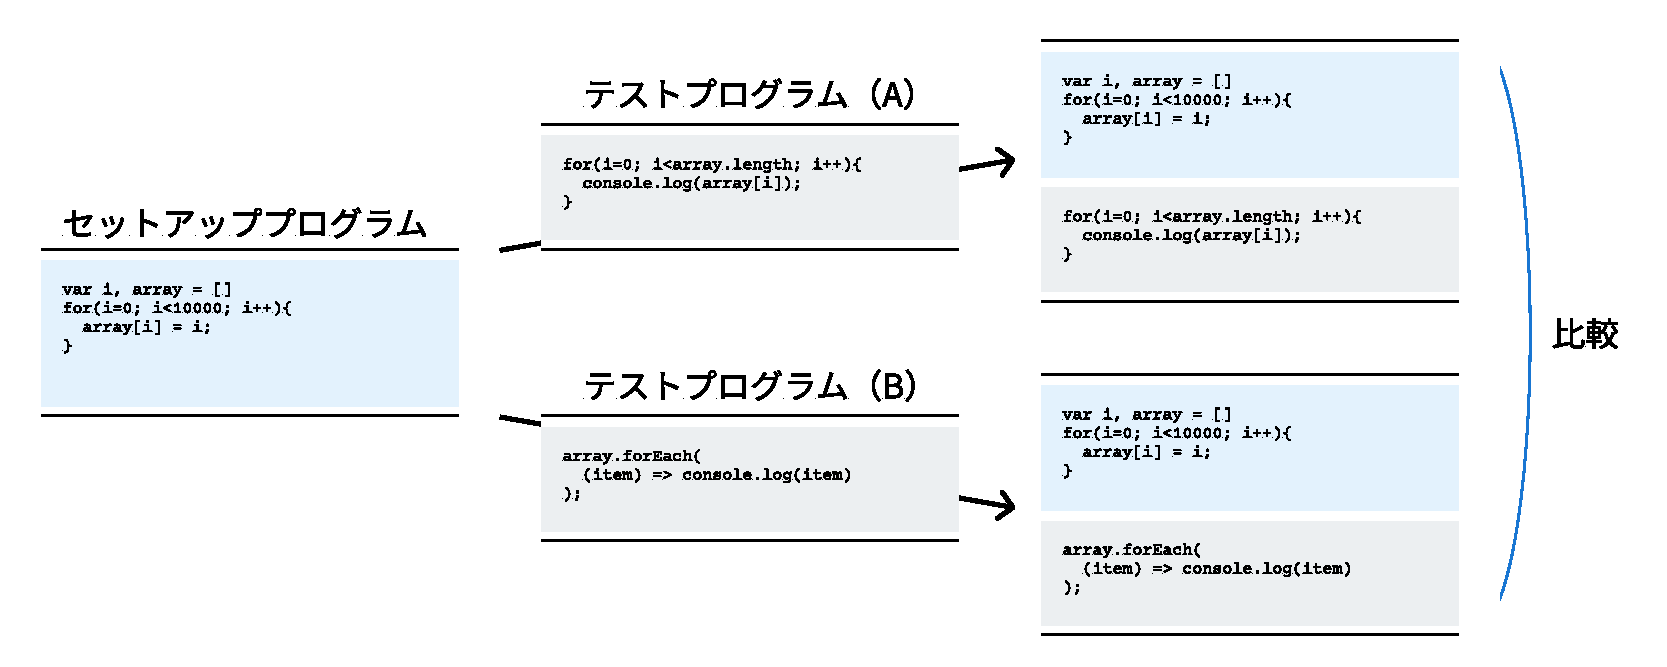
\includegraphics[width=0.96\linewidth]{Omori_fig/concat.pdf}}
\caption{セットアッププログラムとテストプログラムの結合}
\label{fig:concat}
\end{figure}

\begin{figure}[t]
\centerline{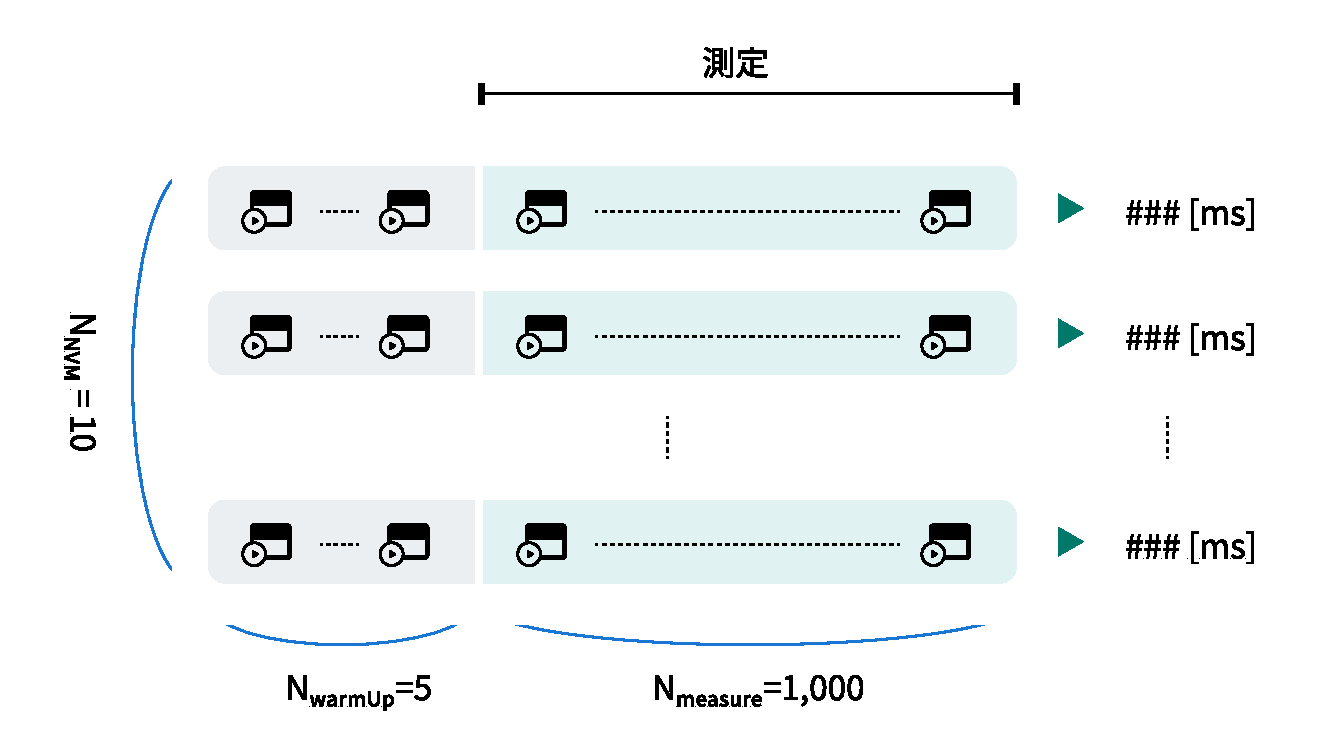
\includegraphics[width=0.768\linewidth]{Omori_fig/measure.pdf}}
\caption{実行時間の測定}
\label{fig-dummy}
\end{figure}

\begin{figure}[t]
\centerline{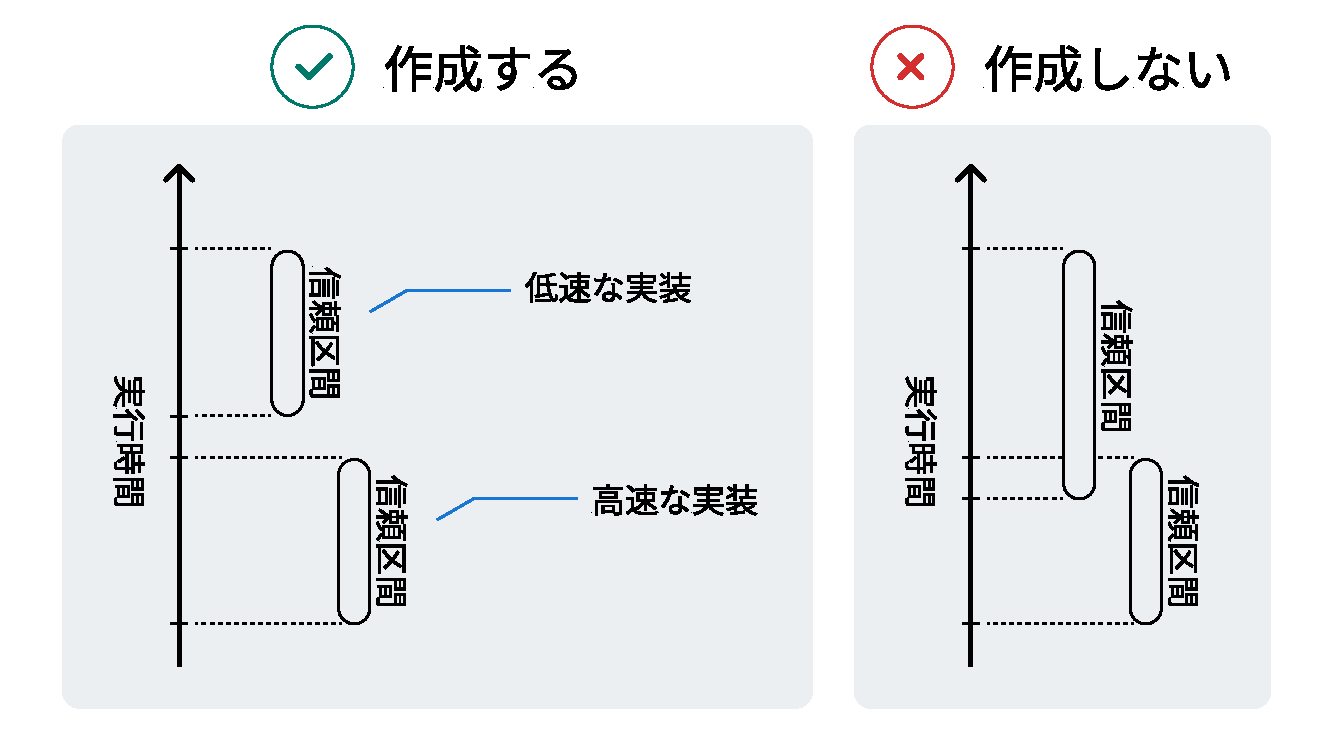
\includegraphics[width=0.768\linewidth]{Omori_fig/compare.pdf}}
\caption{実行時間の比較}
\label{fig-dummy}
\end{figure}


\newpage


%%%%%%%%%%%%%%%%%%%%%%%%%%%%%%%%%%%%%%%%%%%%%%%%%%%%%%%%%%%%%%%%

%%
%% 3.3 データクレンジング
%%

\section{データクレンジング}\label{chapter:dataset:clean}


目視により実装対データセットを調査した結果,可換でない実装対が多く含まれることが分かった.
そのため,実装対の機能的な等価性を検証し,可換でない実装対をデータセットから除外する.
ただし,検証する実装対は68,821組にも及ぶ.
そのため,自動検証手法を用いて実装対の等価性を検証する.


%%%%%%%%%%%%%%%%%%%%%%%%%%%%%%%%%%%%%%%%%%%%%%%%%%%%%%%%%%%%%%%%

%%
%% 3.3.1 既存手法での検証困難性
%%

\subsection{既存手法での検証困難性}


既存の自動検証手法として,テストの自動生成による等価性の検証手法が提案されている\todo{引用}.
しかし,自動生成されたテストでは正しく等価性を判定できない場合がある.
例として,Listing~\ref{unmatched-literals-a}とListing~\ref{unmatched-literals-b}の実装対を示す.
両実装は各々異なる演算を行っているものの,どちらも演算結果を変数に格納することも標準出力に出力することも行わない.
このような実装はマイクロベンチマークに特有であり,自動生成テストでは機能的な等価性を検証できない.

また,ArrayとUint32Arrayのような互換性を持つクラス同士の交換に対しても,型の一致を検証する自動生成テストでは機能的な等価性を検証できない.

以上の理由から,本研究では既存の自動検証手法を用いず,独自の手法で等価性を検証する.


\begin{figure}[t]
\captionsetup{name=Listing}
\hspace{0.04\columnwidth}
\begin{minipage}[b]{0.445\linewidth}
\begin{lstlisting}[
  caption=無関係な実装の比較(A),
  label=non-refactorable-a,
  captionpos=t
]
Math.cos(1);
\end{lstlisting}
\end{minipage}
\hspace{0.059\columnwidth}
\begin{minipage}[b]{0.445\linewidth}
\begin{lstlisting}[
  caption=無関係な実装の比較(B),
  label=non-refactorable-b,
  captionpos=t
]
Math.tan(1);
\end{lstlisting}
\end{minipage}
\end{figure}


%%%%%%%%%%%%%%%%%%%%%%%%%%%%%%%%%%%%%%%%%%%%%%%%%%%%%%%%%%%%%%%%

%%
%% 3.3.2 マイクロベンチマークに対する等価性の検証
%%

\subsection{マイクロベンチマークに対する等価性の検証}


本研究で用いる等価性の検証手法の詳細について,以下に述べる.
本手法を用いた検証の結果,29,809組の可換な実装対を抽出した.


\begin{description}

\item[標準出力の比較]\mbox{}\\
第一に,プログラム間の標準出力を比較し,一致しない実装対を除外する.
実行前にDate.now()関数やMath.random()関数のような参照等価ではない代表的な関数は戻り値を固定する.

結果として,\todo{}件(データクレンジング前データセットの\todo{}\%)の実装対を外した.

\item[終了時の変数格納値の比較]\mbox{}\\
第二に,プログラム終了時の変数格納値を比較し,一致しない実装対を除外する.
具体的には,実装対の両方で同名の変数を同一用途とみなし,すべての変数の格納値が一致する場合,機能的に等しいと判定する.
ただし,実装対の片方でのみ定義された変数については一致を確認せず,両方で定義された変数についてのみ一致を確認する.

また,互換性を持つクラス同士の交換に対応するため,変数格納値はtoString()メソッドを用いて文字列に変換した後,一致を確認する.
ArrayとUint32Arrayのように型が異なる場合でも変換後の文字列は同一であるため,これを利用する.
ただし,連想配列は内部の値に関係なくすべて同一の文字列に変換されるため,別にvalueOf()メソッドを使用する.
toString()メソッドもvalueOf()メソッドもObjectクラスに実装されており,多くのオブジェクトはObjectクラスを継承しているため,これらのメソッドはほとんどの変数格納値に対して呼び出せる.
ただし,例外的にObjectクラスを継承していない値(null)やプログラム終了時点でグローバルスコープから参照できない変数に対しては一致を確認せず,それ以外の変数についてのみ一致を確認する.

結果として,\todo{}件(データクレンジング前データセットの\todo{}\%)の実装対を除外した.

\item[式のみの場合の比較]\mbox{}\\
目視調査の結果,演算結果を変数に格納することも標準出力に出力することも行わない演算の多くは1文のみのテストプログラムに多いことが分かった.
そのため,実装対の両方のテストプログラムが1文(プログラム全体が最後の1文を除いて同一)で,テストプログラムの1文が式として評価できる場合,その演算結果を比較し,一致しない実装対を除外する.

結果として,\todo{}件(データクレンジング前データセットの\todo{}\%)の実装対を除外した.

\end{description}


%%%%%%%%%%%%%%%%%%%%%%%%%%%%%%%%%%%%%%%%%%%%%%%%%%%%%%%%%%%%%%%%

%%
%% 3.4 前処理
%%

\section{前処理}\label{chapter:dataset:prep}


%%%%%%%%%%%%%%%%%%%%%%%%%%%%%%%%%%%%%%%%%%%%%%%%%%%%%%%%%%%%%%%%

%%
%% 3.4.1 使用されていない変数・関数の除去
%%

\subsection{使用されていない変数・関数の除去}


マイクロベンチマークでは共通のセットアッププログラムを用いるため,各テストプログラムで使用される変数や関数がすべて記述される.
そのため,セットアッププログラムとテストプログラムの結合時,結合するテストプログラムでは使用されない変数や関数がセットアッププログラムに含まれる場合がある.
機能に無関係な変数や関数の含有は学習の妨げになると考えられるため,結合したプログラムから使用されない変数や関数を除去する.
プログラム内での使用有無は,静的解析ツールESLintを用いて判定する.


\begin{figure}[t]
\captionsetup{name=Listing}
\hspace{0.04\columnwidth}
\begin{minipage}[b]{0.96\linewidth}
\begin{lstlisting}[
  caption=セットアッププログラム,
  label=microbenchmark-setup,
  captionpos=t
]
var i, array = [];
for(i=0; i<10000; i++){
  array[i] = i;
}

const a = () => {
  for(i=0; i<array.length; i++){
    console.log(array[i]);
  }
}

const b = () => {
  array.forEach(
    (item) => console.log(item)
  );
}
\end{lstlisting}
\end{minipage}

\hspace{0.04\columnwidth}
\begin{minipage}[b]{0.445\linewidth}
\begin{lstlisting}[
  caption=テストプログラムA,
  label=microbenchmark-test-1,
  captionpos=t,
  firstnumber=14
]
a();
\end{lstlisting}
\end{minipage}
\hspace{0.059\columnwidth}
\begin{minipage}[b]{0.445\linewidth}
\begin{lstlisting}[
  caption=テストプログラムB,
  label=microbenchmark-test-2,
  captionpos=t,
  firstnumber=14
]
b();
\end{lstlisting}
\end{minipage}
\end{figure}


\begin{figure}[t]
\captionsetup{name=Listing}
\hspace{0.04\columnwidth}
\begin{minipage}[b]{0.445\linewidth}
\begin{lstlisting}[
  caption=テストプログラムA(結合後),
  label=unmatched-literals-a,
  captionpos=t
]
var i, array = [];
for(i=0; i<10000; i++){
    array[i] = i;
}

const a = () => {
for(i=0; i<array.length; i++)
    console.log(array[i]);
}

a();
\end{lstlisting}
\end{minipage}
\hspace{0.059\columnwidth}
\begin{minipage}[b]{0.445\linewidth}
\begin{lstlisting}[
  caption=テストプログラムB(結合後),
  label=unmatched-literals-b,
  captionpos=t
]
var i, array = [];
for(i=0; i<10000; i++){
    array[i] = i;
}

const b = () => {
array.forEach(
  (item) => console.log(item)
);

b();
\end{lstlisting}
\end{minipage}
\end{figure}


%%%%%%%%%%%%%%%%%%%%%%%%%%%%%%%%%%%%%%%%%%%%%%%%%%%%%%%%%%%%%%%%

%%
%% 3.4.2 抽象化
%%

\subsection{抽象化}


一般に,プログラム自動修正モデルの学習データセットは,モデルの汎化性能を高めるためプログラム中の変数名や関数名,リテラルを抽象化されることが多い\todo{引用}.
本研究でも同様に実装対データセットを抽象化する.
ただし,一般的なプログラム自動修正モデルがバグ修正を目的としているのに対して本研究のモデルはリファクタリングを目的としている.
そのため,一般的な学習データセットの抽象化手法とは異なる基準により,特定のトークンのみを抽象化する.
抽象化手法の詳細について,以下に述べる.


\begin{description}

\item[変数名]\mbox{}\\
プログラム中で宣言されている変数のみ抽象化する.
抽象化後の変数名は,VAR\_1,VAR\_2のように連番で区別する.
また,実装対の両方に共通する変数名は,同一の変数名に抽象化する.
Listing~\ref{microbenchmark-test-1}中のconsoleオブジェクト等,プログラム中で明示的に宣言されていない変数(グローバルオブジェクト)は常に固有の名前を持つため,抽象化しない.

\item[関数名]\mbox{}\\
変数名と同様に,プログラム中で宣言されている関数のみを抽象化する.
抽象化後の関数名は,FUNCTION\_1,FUNCTION\_2のように連番で区別する.

\item[リテラル]\mbox{}\\
リテラルを抽象化することで修正を捉えられなくなる場合があるため,すべてのリテラルを抽象化しない.
例として,Listing~\ref{unmatched-literals-a}とListing~\ref{unmatched-literals-b}の実装対を示す.
両実装はどちらも小数n=1.234から小数第2位までの概数(1.23)を求める.
そのため,両実装の引数は異なる(2と100)ものの,暗黙的な対応関係(\begin{math}\log_{10} 100=2\end{math})を持つ.
このような場合にはリテラルの抽象化により,暗黙的な対応関係が失われる.

\end{description}


\begin{figure}[t]
\captionsetup{name=Listing}
\hspace{0.04\columnwidth}
\begin{minipage}[b]{0.445\linewidth}
\begin{lstlisting}[
  caption=リテラルが共通しない実装(A),
  label=unmatched-literals-a,
  captionpos=t
]
let n = 1.234;
n.toFixed(2);
\end{lstlisting}
\end{minipage}
\hspace{0.059\columnwidth}
\begin{minipage}[b]{0.445\linewidth}
\begin{lstlisting}[
  caption=リテラルが共通しない実装(B),
  label=unmatched-literals-b,
  captionpos=t
]
let n = 1.234;
Math.round(n*100)/100;
\end{lstlisting}
\end{minipage}
\end{figure}


例として,プログラム\ref{microbenchmark-test-1}と\ref{microbenchmark-test-2}を抽象化した結果をListing~\ref{abstract-a}と\ref{abstract-b}に示す.


\begin{figure}[t]
\captionsetup{name=Listing}
\hspace{0.04\columnwidth}
\begin{minipage}[b]{0.96\linewidth}
\begin{lstlisting}[
  caption=テストプログラムA(抽象化後),
  label=abstract-a,
  captionpos=t
]
var VAR_1, VAR_2 = [];
for(VAR_1=0; VAR_1<10000; VAR_1++){
    VAR_2[VAR_1] = VAR_1;
}

for(VAR_1=0; VAR_1<VAR_2.length; VAR_1++){
    console.log(VAR_2[VAR_1]);
}
\end{lstlisting}
\end{minipage}
\end{figure}

\begin{figure}[t]
\captionsetup{name=Listing}
\hspace{0.04\columnwidth}
\begin{minipage}[b]{0.96\linewidth}
\begin{lstlisting}[
  caption=テストプログラムB(抽象化後),
  label=abstract-b,
  captionpos=t
]
var VAR_1, VAR_2 = [];
for(VAR_1=0; VAR_1<10000; VAR_1++){
    VAR_2[VAR_1] = VAR_1;
}

VAR_2.forEach(
  (VAR_3) => console.log(VAR_3)
);
\end{lstlisting}
\end{minipage}
\end{figure}


%%%%%%%%%%%%%%%%%%%%%%%%%%%%%%%%%%%%%%%%%%%%%%%%%%%%%%%%%%%%%%%%

%%
%% 4 モデル構築
%%

\chapter{自動リファクタリングモデル}\label{chapter:model}


本研究では,深層学習とパターンマッチを用いたプログラム自動修正モデルを各々作成する.
深層学習モデルとパターンマッチモデルはどちらも代表的な自動修正モデルであるが,互いに異なる手法でプログラムを修正する.

深層学習モデルは,入力されたプログラム全体の文脈に基づいてプログラムを修正する.
そのため,特に動的型付け言語に対しては,オブジェクトの型を文脈から推測することでパターンマッチモデルよりも柔軟に修正できると考える.
一方で,入力プログラムが長く複雑になると文脈を解釈しきれず,修正性能が低下する.

パターンマッチモデルは,プログラム全体の文脈に関係なく,パターンに合致する実装箇所を限局・修正するため,入力プログラムが長く複雑な場合であっても,深層学習モデルより頑健に修正できることが期待される.
一方で,型推論が困難な動的型付け言語に対しては,パターンを適切に抽象化できないため,誤検出や検出もれが多く発生する.

本研究では,実装対データセットを用いて特徴の異なる2種のモデルを作成し,各々の高速化性能を調査する.


%%%%%%%%%%%%%%%%%%%%%%%%%%%%%%%%%%%%%%%%%%%%%%%%%%%%%%%%%%%%%%%%

%%
%% 4.1 深層学習モデル
%%

\section{深層学習モデル}


深層学習モデルを用いた代表的なプログラム自動修正手法には,プログラムの修正を文章補完や文書翻訳のタスクとして学習させる手法がある\todo{引用}.
文章補完タスクを用いた自動修正では,修正箇所をマスクしたプログラムを入力し,マスクされた箇所の実装を周辺の文脈から補完したプログラムを出力するようにモデルを学習させる.
文書翻訳タスクを用いた自動修正では,プログラムを入力し,一部または全部を修正したプログラムを出力するようにモデルを学習させる.

マイクロベンチマークの多くは非常に小さなプログラムであるため,修正箇所をマスクするとプログラムのほとんどが隠される.
そのため,文章補完タスクでは周辺の文脈が不足し,プログラムの修正方法を十分に学習できないと考える.
そこで,本研究では文書翻訳タスクを用いて深層学習モデルを作成する.

また,深層学習に用いる大規模言語モデルには,2024年時点で最新のモデルであるChatGPT-4o\footnote{\url{https://openai.com/index/hello-gpt-4o/}}とCodeT5+\cite{Wang_2023}を用いる.

ChatGPT-4oは2023年10月までの広範なテキストデータによって学習された最新の大規模言語モデルであり,複数のプログラミング言語のみならず,広範な自然言語の変換にも用いられる大規模言語モデルである.
ChatGPT-4oの学習時と検証時には,入力として自然言語(英語)による指示文と修正元プログラムからなるプロンプトを与える.
プロンプトは\cite{{Ishizue_2024}}を参考に作成した.
作成したプロンプトをListing~\ref{prompt}に示す.

CodeT5+はオープンソースソフトウェアの開発履歴からプログラミング言語間,自然言語・プログラミング言語間の変換タスクを膨大に学習した最新の大規模言語モデルである.
本研究ではCodeT5+を同一プログラミング言語間の変換タスクに用いる.
また,CodeT5+の入力には修正元プログラムのみを与え,自然言語によるプロンプトは与えない.


\begin{figure}[t]
\captionsetup{name=Listing}
\hspace{0.04\columnwidth}
\begin{minipage}[b]{0.96\linewidth}
\begin{lstlisting}[
  caption=プロンプト,
  label=prompt,
  captionpos=t,
  breaklines=true,
  breakindent=-1mm,
  numbers=none
]
As a JavaScript programming expert, your goal is to make the code faster. Make only necessary modifications to the code and keep its essence. Answer only the code.
\end{lstlisting}
\end{minipage}
\end{figure}


両モデルは,どちらも高速化のためのリファクタリングに特化したモデルではない.
本研究では,実装対データセットを用いて両モデルをファインチューニングし,高速化修正に特化したモデルを作成する.
ファインチューニングの際には,実装対のうち,実行時間の長いプログラムを入力し,実行時間の短いプログラムを出力するように学習させる.
各々の大規模言語モデルのファインチューニング時のハイパーパラメータを表~\ref{table:model:params}に示す.
ChatGPT-4oのハイパーパラメータについては,学習時に自動的に決定される値を用いた.
また,CodeT5+のハイパーパラメータについて,学習率はWangら\cite{Wang_2023}がファインチューニング時に用いている値,エポック数はWangらが公開しているCodeT5+公式リポジトリ\footnote{\url{https://github.com/salesforce/CodeT5}}のデフォルト値,バッチサイズは本研究のモデル作成環境の制約から値を決定した.
\todo{最大トークン長は実装対データセット内のトークン長の分布に基づいて決めた気がする}

本研究では,深層学習モデルのファインチューニングに検証データセットを用いない.
\ref{chapter:dataset}章で作成した実装対データセットは,単一のマイクロベンチマーク内では最も高速な実装への修正であるものの,同じ機能に関する他のマイクロベンチマーク内にさらに高速な実装が含まれている可能性や,セットアッププログラム等の比較対象以外の実装が同時に修正される可能性が考えられる.
高速化修正の成否が判定困難であるため,本研究では検証データセットを用いない.


% 変数名の抽象化を直す.


\begin{table}[t]
\caption{深層学習モデルのハイパーパラメータ}
\label{table:model:params}
\centering
\begin{tabular}{lrrrr}
\hline
モデル & エポック数 & バッチサイズ & 学習率 & 最大トークン長 \\
\hline
ChatGPT-4o & 1 & 15 & 1.8 & 512 \\
CodeT5+ & 10 & 8 & 2e-5 & 512 \\
\hline
\end{tabular}
\end{table}


%%%%%%%%%%%%%%%%%%%%%%%%%%%%%%%%%%%%%%%%%%%%%%%%%%%%%%%%%%%%%%%%

%%
%% 4.2 パターンマッチモデル
%%

\section{パターンマッチモデル}


%%%%%%%%%%%%%%%%%%%%%%%%%%%%%%%%%%%%%%%%%%%%%%%%%%%%%%%%%%%%%%%%

%%
%% 4.2.1 抽象構文木に基づくパターンマッチの利点
%%

\subsection{抽象構文木に基づくパターンマッチの利点}


本研究では,抽象構文木に基づいて実装対の差分をパターン化する.
既存のパターンマッチ手法では,差分を行単位で抽出してパターン化することが多い\todo{引用}.
しかし,しばしばリファクタリングは行単位よりも細かな粒度で行われる.
例として,Listing~\ref{unmatched-literals-a}とListing~\ref{unmatched-literals-b}の実装差分から,n.toFixed(2);という文からMath.round(n*100)/100;という文への変更によってプログラムを高速化するパターンを作成できる.
しかし,両実装はどちらも演算結果の保存や出力等を行っておらず,作成パターンが実用的なプログラムにそのまま出現するとは考え難い.
Listing~\ref{unmatched-literals-a}とListing~\ref{unmatched-literals-b}の場合は文ではなくメソッド(関数)単位で差分を抽出し,Listing~\ref{unmatched-literals-c}のようにtoFixed()メソッドが代入式や条件式の中に出現する場合にも対応するべきである.
そこで,本研究では,抽象構文木を用いることで行単位よりも細かな粒度で差分をパターン化する.


\begin{figure}[t]
\captionsetup{name=Listing}
\hspace{0.04\columnwidth}
\begin{minipage}[b]{0.96\linewidth}
\begin{lstlisting}[
  caption=行単位のパターンマッチでは検出できない例,
  label=unmatched-literals-c,
  captionpos=t
]
let n = 1.234;
let round_n = n.toFixed(2); // 元の実装と異なり,値を代入している
\end{lstlisting}
\end{minipage}
\end{figure}


%%%%%%%%%%%%%%%%%%%%%%%%%%%%%%%%%%%%%%%%%%%%%%%%%%%%%%%%%%%%%%%%

%%
%% 4.2.2 抽象構文木に基づくパターンマッチ
%%

\subsection{抽象構文木に基づくパターンマッチ}


% パターンの作成
実装対の内,より低速な実装を修正元,より高速な実装を修正先として,両実装の差分を抽出する.
差分抽出時は両実装を抽象構文木に変換し,Gumtree\cite{Falleri_2014}を用いて差分を特定する.
差分抽出の例を図\ref{fig:pattern:create}に示す.
図\ref{fig:pattern:create}のように,抽出した差分は修正元・修正先の両実装で同一の親ノードを持ち,ソースコード上の位置によって一意に順序が定まる\footnote{部分木を別の位置に移動する修正は「部分木の削除」と「部分木の追加」の2差分として別個に検出される.}.
また,差分(部分木の対)は以下の3種類のいずれかの変更に分類される.


\begin{description}

\item[部分木の変更]\mbox{}\\
修正元の実装から部分木を削除し,修正先の実装に異なる部分木を追加する修正.

\item[部分木の削除]\mbox{}\\
修正元の実装から部分木を削除する修正.

\item[部分木の追加]\mbox{}\\
修正先の実装に部分木を追加する修正.
追加関係にある差分からは,部分木の追加位置を特定できない.
そのため,追加関係にある差分を含む実装対からはパターンを作成しない.

\end{description}


修正元・修正先プログラムから抽出した部分木の変数・関数・リテラルノードを抽象化し,修正元・修正先パターンを作成する.
抽象化手法の詳細について,以下に述べる.
結果として,実装対データセットから\todo{}件のパターン対を作成した.\todo{}


\begin{description}

\item[変数ノード]\mbox{}\\
変数ノードは,変数やリテラルを含む任意の式として抽象化する.
ただし,パターン内の同名の変数ノードは,すべて同一の式にのみ一致する.

\item[関数ノード]\mbox{}\\
関数ノードは,アロー関数を含む任意の関数として抽象化する.
ただし,パターン内の同名の関数ノードは,すべて同一の関数にのみ一致する.

\item[リテラルノード]\mbox{}\\
リテラルノードは,型が一致する任意のリテラルとして抽象化する.
値が一致しない場合でも,型が一致していれば一致する.

\end{description}


% パターンの適用
パターンの適用時には,入力プログラムから修正元パターンを検出し,検出箇所を修正先パターンに変換する.
パターン検出の例を図\ref{fig:pattern:match}に,パターン変換の例を図\ref{fig:pattern:repair}に示す.
修正元パターンの検出時は,入力プログラムが修正元パターン内のすべての部分木を同じ順序で含む場合のみ修正元パターンを検出する.
また,修正先パターン内の変数ノードや関数ノードは,同名のノードが修正元パターンに含まれる場合,修正元パターン内のノードとマッチした入力プログラム内の部分木に書き換える.
同名のノードが修正元パターンに含まれない場合,修正先パターン内の変数・関数はそのまま用いる.


\begin{figure}[t]
\centerline{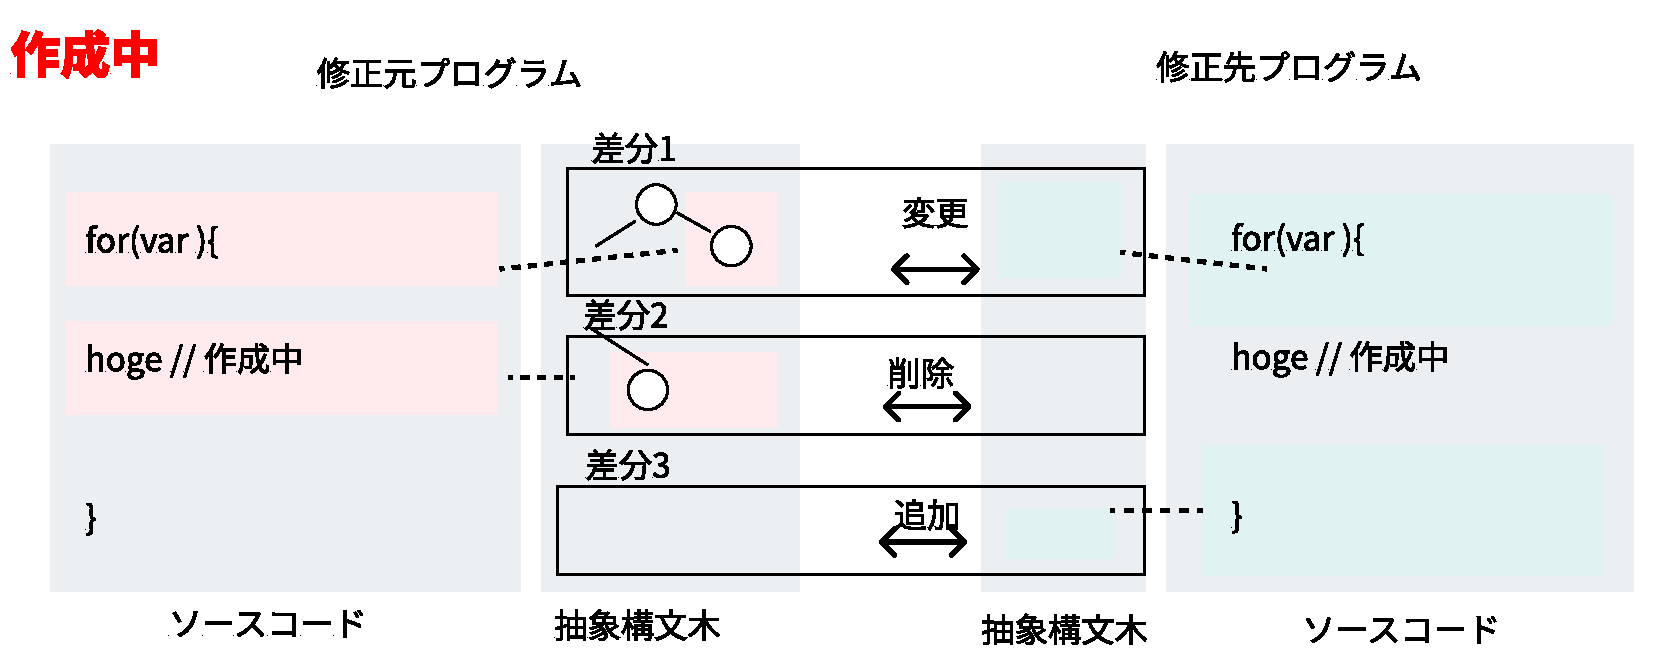
\includegraphics[width=0.8\linewidth]{Omori_fig/pattern-create.pdf}}
\caption{パターンの作成}
\label{fig:pattern:create}
\end{figure}

\begin{figure}[t]
\centerline{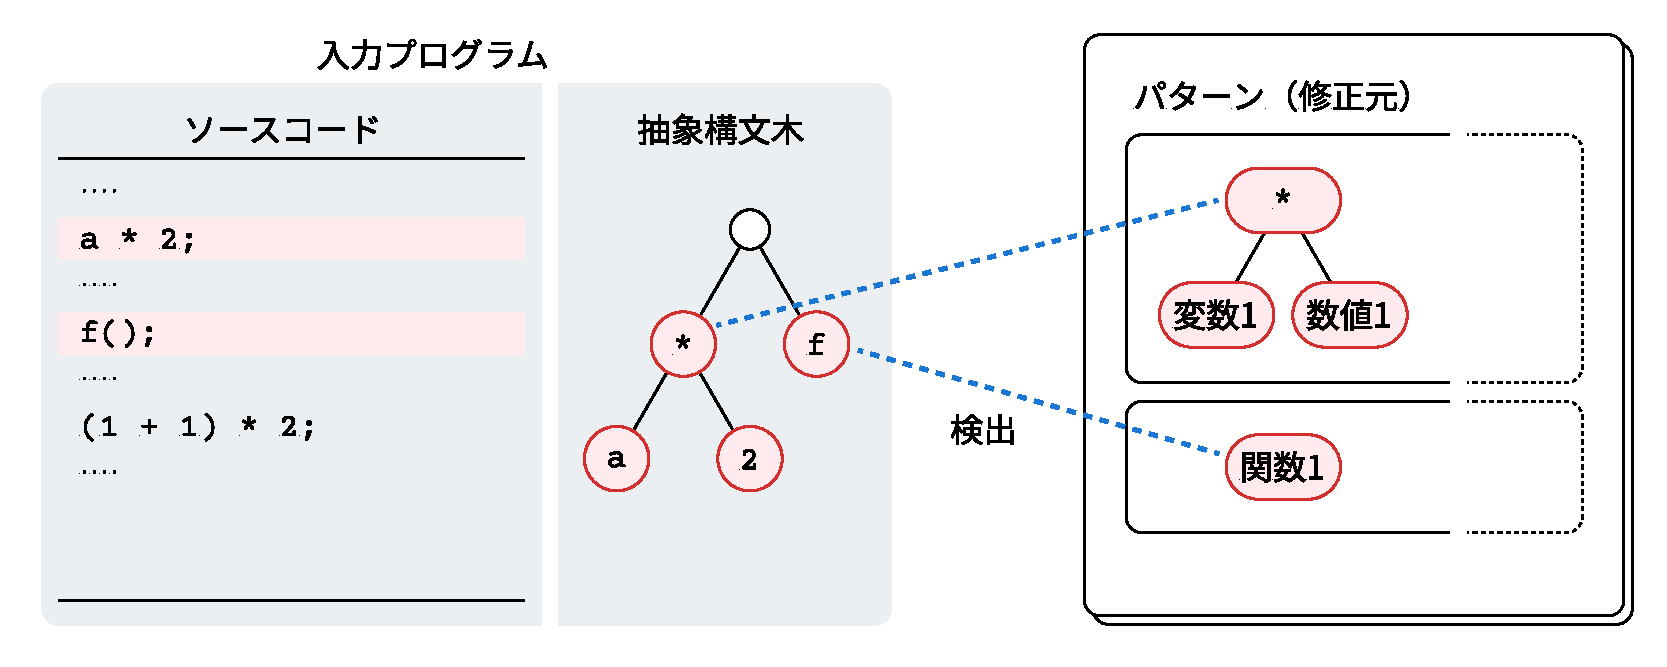
\includegraphics[width=0.8\linewidth]{Omori_fig/pattern-match.pdf}}
\caption{パターンの検出}
\label{fig:pattern:match}
\end{figure}

\begin{figure}[t]
\centerline{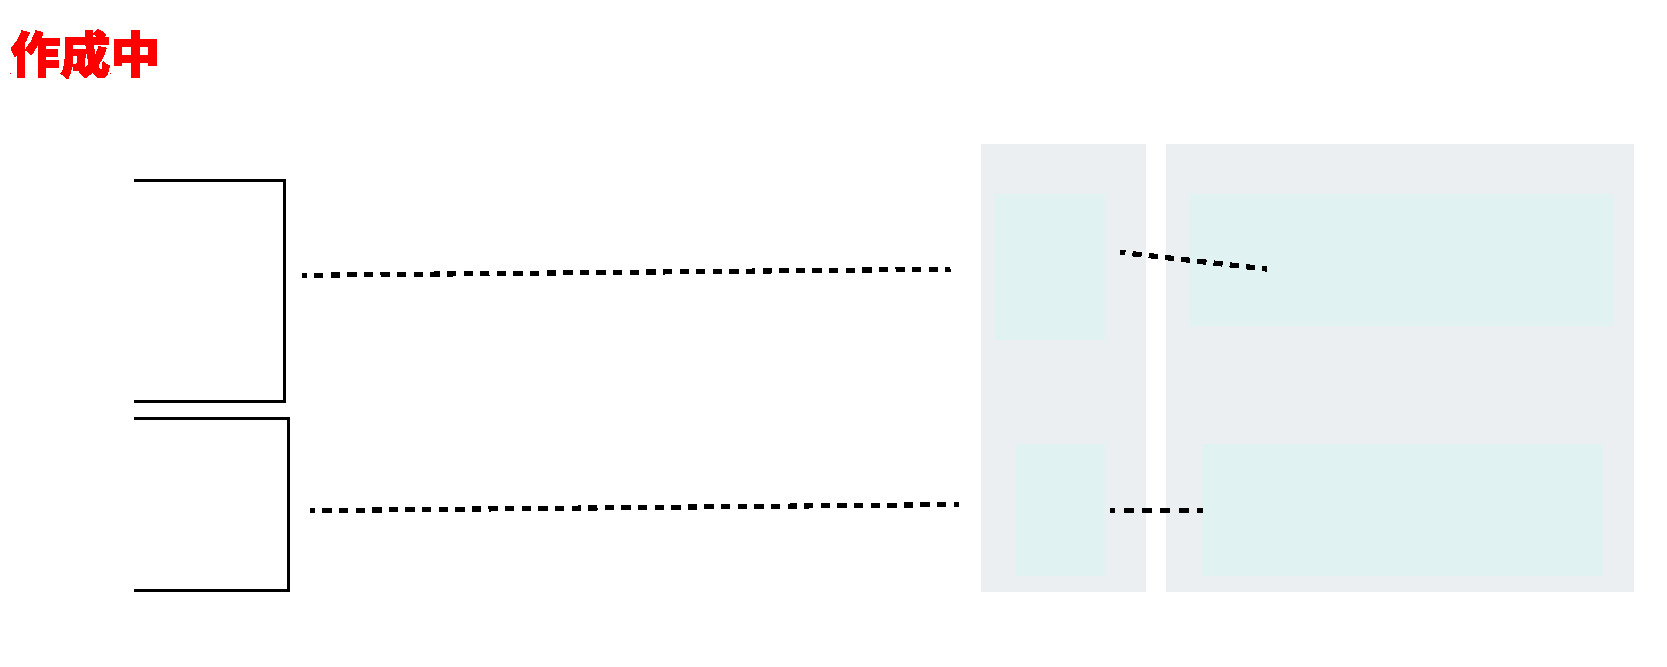
\includegraphics[width=0.8\linewidth]{Omori_fig/pattern-repair.pdf}}
\caption{パターンの適用}
\label{fig:pattern:repair}
\end{figure}


%%%%%%%%%%%%%%%%%%%%%%%%%%%%%%%%%%%%%%%%%%%%%%%%%%%%%%%%%%%%%%%%

%%
%% 5 マイクロベンチマークに対する修正性能評価
%%

\chapter{マイクロベンチマークに対する修正性能評価}\label{chapter:eval-1}


%%%%%%%%%%%%%%%%%%%%%%%%%%%%%%%%%%%%%%%%%%%%%%%%%%%%%%%%%%%%%%%%

%%
%% 5.1 実験方法
%%

\section{実験方法}


本章では,学習時と同じ実装対データセットを用いて提案モデルと既存モデルの高速化性能を比較する.
各モデルが生成したプログラムは,\ref{chapter:dataset:clean}節で作成したアルゴリズムを用いて入力プログラムとの等価性を判定した上で,\ref{chapter:dataset:measure}節と同様の手法で高速化の成否を統計的に判定する.


%%%%%%%%%%%%%%%%%%%%%%%%%%%%%%%%%%%%%%%%%%%%%%%%%%%%%%%%%%%%%%%%

%%
%% 5.1.1 評価データセット
%%

\subsection{評価データセット}


評価データセットには,実装対データセットを学習用途と検証用途に分割して用いる.
学習用途には実装対データセットの8割を用い,提案モデルに学習させる.
検証用途には残りの2割を用い,提案モデルと既存モデルの高速化性能を測定する.
検証時には,実装対の内,より低速な実装を入力する.


%%%%%%%%%%%%%%%%%%%%%%%%%%%%%%%%%%%%%%%%%%%%%%%%%%%%%%%%%%%%%%%%

%%
%% 5.1.2 評価対象モデル
%%

\subsection{評価対象モデル}


本研究では,提案モデルの性能を評価するためのベースラインとして,追加のファインチューニングを行わないCodeT5+およびChatGPT-4oモデルを用いる.
さらに,実装対データセットの作成時にデータクレンジングを行わないモデルを作成し,本研究で独自に行ったデータクレンジングの有効性を調査する.
したがって,本章では表~\ref{table:eval-1:result-test-fast}に示す8件のモデルの性能を比較する.


\begin{figure}[t]
\centerline{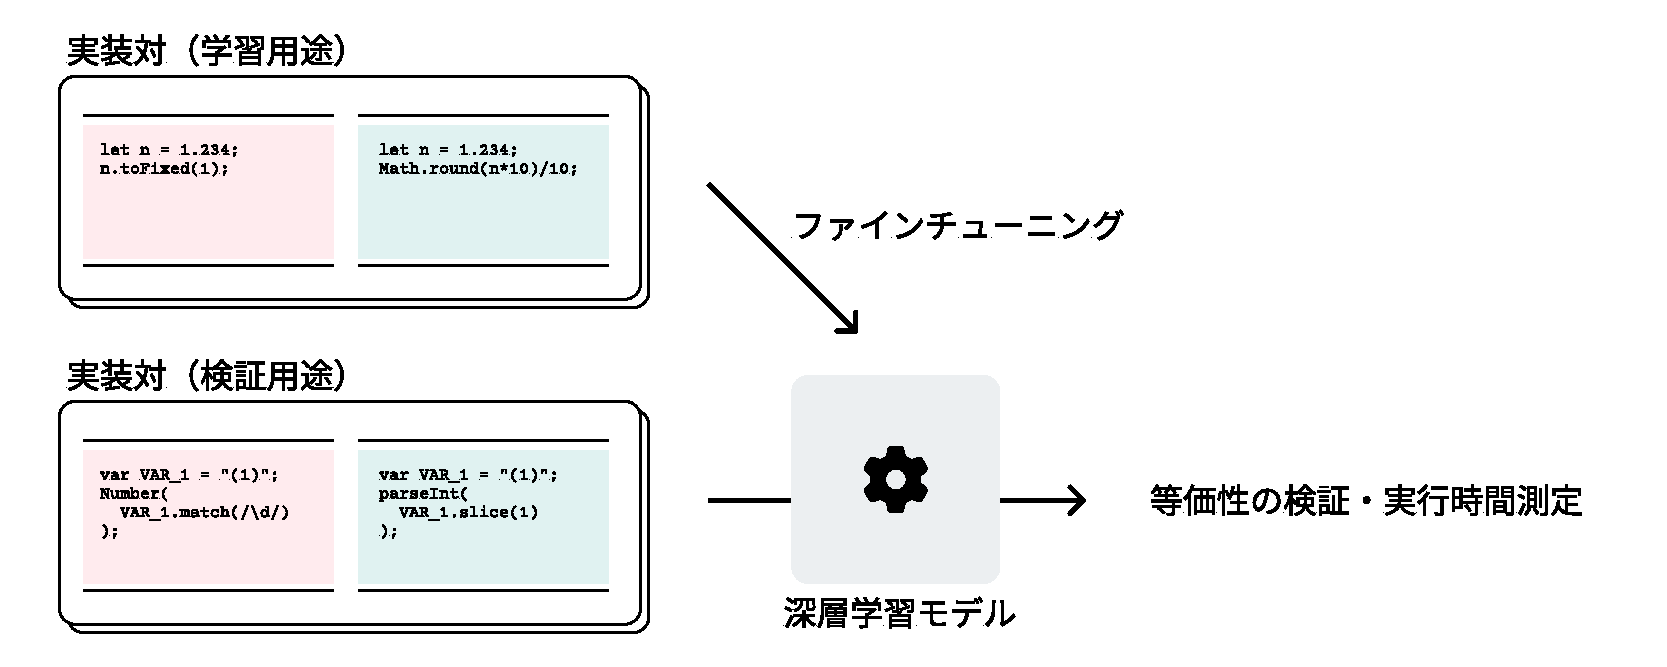
\includegraphics[width=0.8\linewidth]{Omori_fig/eval-1.pdf}}
\caption{overview}
\label{fig-dummy}
\end{figure}


%%%%%%%%%%%%%%%%%%%%%%%%%%%%%%%%%%%%%%%%%%%%%%%%%%%%%%%%%%%%%%%%

%%
%% 5.2 結果
%%

\section{結果}\label{sec:result}


結果を表\ref{table:eval-1:result-test-fast}に示す.
表\ref{table:eval-1:result-test-fast}より,検証データセット5,962件のうち,パターンマッチモデルは最大1,638件(27.5\%),深層学習モデルは最大2,834件(47.5\%)の入力プログラムに対して高速化に成功した.
特に,実装対データセットを用いてファインチューニングを行ったCodeT5+モデルは,ファインチューニングを行わないChatGPT-4oモデルと比べ,11.0ポイント多くプログラムの高速化に成功した.
また,実装対データセットのデータクレンジング有無によって,パターンマッチモデルでは大きく,ChatGPT-4oモデルではわずかに修正成功率が増加した.
本実験ではパターンマッチモデルによる修正時,マッチするパターンの組み合わせによって複数の修正プログラムが出力できる場合でも,ランダムに抽出された最大10件のプログラムのみを出力する.
したがって,データクレンジング前の実装対データセットに含まれる等価でない実装対から,多くの(等価でない)パターンが作成されたため,データクレンジング後よりも誤検出が多かったと考えられる.
一方でCodeT5+モデルではわずかに修正成功率が低下したことから,CodeT5+モデルではデータクレンジングによる学習データセット数の減少が,等価でない実装対の混入よりも学習に影響を与えると考えられる.
ChatGPT-4oモデルではデータクレンジングによる修正成功率の低下が見られないため,より大規模なデータセットで事前学習された大規模言語モデルを用いることでデータセット数減少による性能低下を防ぐことができると考えられる.

以下,各節において各モデルの生成プログラムを分析する.
ただし,ファインチューニング前のCodeT5+モデルはすべての入力プログラムに対して入力と完全に同じプログラムを出力したため,議論から除外する.


\begin{table}[t]
\caption{実験結果}
\label{table:eval-1:result-test-fast}
\centering
\begin{tabular}{lcc|rr}
\hline
モデル & ファインチューニング & データクレンジング & 等価 [件] & 等価かつ高速 [件] \\
\hline
パターンマッチ & - & なし & 5,711 & 330 \\ % 7
パターンマッチ & - & あり & 5,187 & 1,638 \\ % 6
ChatGPT-4o & なし & - & 5,285 & 2,180 \\ % 3
ChatGPT-4o & あり & なし & 5,066 & 2,627 \\ % 5
ChatGPT-4o & あり & あり & 5,501 & 2,750 \\ % 4
CodeT5+ & なし & - & 0 & 0 \\ % 0
CodeT5+ & あり & なし & 5,302 & 2,938 \\ % 2
CodeT5+ & あり & あり & 5,473 & 2,834 \\ % 1
\hline
\end{tabular}
\end{table}


%%%%%%%%%%%%%%%%%%%%%%%%%%%%%%%%%%%%%%%%%%%%%%%%%%%%%%%%%%%%%%%%

%%
%% 5.2.1 パターンマッチ
%%

\subsection{パターンマッチ}


Listing~\ref{listing:eval-1:result-pattern-success-input},Listing~\ref{listing:eval-1:result-pattern-success-output}にパターンマッチモデルによる生成プログラムの一例を示す.
Listing~\ref{listing:eval-1:result-pattern-success-input},Listing~\ref{listing:eval-1:result-pattern-success-output}は入力プログラムおよび,データクレンジング後の実装対データセットを学習したパターンマッチモデルの出力プログラムである.
また,データクレンジング前の実装対データセットを学習したパターンマッチモデルであっても,Listing~\ref{listing:eval-1:result-pattern-success-output}と同じプログラムを出力することを確認した.
各実装は,入力プログラムとパターンマッチモデル(データクレンジング前・後の両方)が生成した実装であり,いずれも現在の時刻をミリ秒単位で求める実装である.
入力(Listing~\ref{listing:eval-1:result-pattern-success-input})ではDateインスタンスを作成し,getMilliseconds()メソッドを呼び出すことで機能を実装しているが,生成プログラム(Listing~\ref{listing:eval-1:result-pattern-success-output})では静的メソッドであるDate.now()メソッドを用いることで実装を高速化している.


\begin{figure}[t]
\captionsetup{name=Listing}
\hspace{0.04\columnwidth}
\begin{minipage}[b]{0.96\linewidth}
\begin{lstlisting}[
  caption=パターンマッチによる成功例(入力),
  label=listing:eval-1:result-pattern-success-input,
  captionpos=t
]
new Date().getMilliseconds();
\end{lstlisting}
\end{minipage}

\hspace{0.04\columnwidth}
\begin{minipage}[b]{0.96\linewidth}
\begin{lstlisting}[
  caption=パターンマッチによる成功例(出力),
  label=listing:eval-1:result-pattern-success-output,
  captionpos=t
]
Date.now() % 1000;
\end{lstlisting}
\end{minipage}
\end{figure}


%%%%%%%%%%%%%%%%%%%%%%%%%%%%%%%%%%%%%%%%%%%%%%%%%%%%%%%%%%%%%%%%

%%
%% 5.2.2 ChatGPT-4o
%%

\subsection{ChatGPT-4o}


Listing~\ref{result-chatgpt-success-input}とListing~\ref{result-chatgpt-success-output}にChatGPT-4oをファインチューニングしたモデルによる生成プログラムの一例を示す.
Listing~\ref{result-chatgpt-success-input}とListing~\ref{result-chatgpt-success-output}は入力プログラムおよび,データクレンジング後の実装対データセットを学習したChatGPT-4oモデルの出力プログラムである.
Listing~\ref{result-chatgpt-success-input}とListing~\ref{result-chatgpt-success-output}は,どちらもユーザ定義関数FUNCTION\_1()内で引数VAR\_3がVAR\_1("hi")またはVAR\_2("hello")と一致するかどうかを判定するプログラムである.
入力プログラム(Listing~\ref{result-chatgpt-success-input})では,VAR\_1とVAR\_2を配列に格納し,includes()メソッドを用いて配列がVAR\_3と一致する要素を含むか判定している.
一方で,修正プログラム(Listing~\ref{result-chatgpt-success-output})では,配列を作成する代わりにVAR\_1,VAR\_2との一致を各々判定することで高速化している.


\begin{figure}[t]
\captionsetup{name=Listing}
\hspace{0.04\columnwidth}
\begin{minipage}[b]{0.96\linewidth}
\begin{lstlisting}[
  caption=ファインチューニング済みChatGPT-4oによる成功例(入力),
  label=result-chatgpt-success-input,
  captionpos=t
]
const VAR_1 = "hi";
const VAR_2 = "hello";

function FUNCTION_1(VAR_3) {
  return [VAR_1, VAR_2].includes(VAR_3);
}

FUNCTION_1("hi");
\end{lstlisting}
\end{minipage}

\hspace{0.04\columnwidth}
\begin{minipage}[b]{0.96\linewidth}
\begin{lstlisting}[
  caption=ファインチューニング済みChatGPT-4oによる成功例(出力),
  label=result-chatgpt-success-output,
  captionpos=t
]
const VAR_1 = "hi";
const VAR_2 = "hello";

function FUNCTION_1(VAR_3) {
  return VAR_3 === VAR_1 || VAR_3 === VAR_2;
}

FUNCTION_1("hi");
\end{lstlisting}
\end{minipage}
\end{figure}


%%%%%%%%%%%%%%%%%%%%%%%%%%%%%%%%%%%%%%%%%%%%%%%%%%%%%%%%%%%%%%%%

%%
%% 5.2.3 CodeT5+
%%

\subsection{CodeT5+}


Listing~\ref{result-codet5-success-input},Listing~\ref{result-codet5-success-output}にCodeT5+をファインチューニングしたモデルによる生成プログラムの一例を示す.
Listing~\ref{result-codet5-success-input}とListing~\ref{result-codet5-success-output}は入力プログラムおよび,データクレンジング後の実装対データセットを学習したCodeT5+モデルの出力プログラムである.
Listing~\ref{result-codet5-success-input}とListing~\ref{result-codet5-success-output}は,どちらも配列VAR\_1とVAR\_2を結合するプログラムである.
入力プログラム(Listing~\ref{result-codet5-success-input})では,reduce()メソッドを用いてVAR\_2の要素を順にVAR\_1に格納している.
一方で,修正プログラム(Listing~\ref{result-codet5-success-output})では,concat()メソッドを用いて配列を結合することで実装を高速化している.


\begin{figure}[t]
\captionsetup{name=Listing}
\hspace{0.04\columnwidth}
\begin{minipage}[b]{0.96\linewidth}
\begin{lstlisting}[
  caption=ファインチューニング済みCodeT5+による成功例(入力),
  label=result-codet5-success-input,
  captionpos=t
]
var VAR_1 = [1, 2, 3, 4, 5, 6, 7, 8, 9];
var VAR_2 = ["foo", "bar", "baz", "bam", "bun", "fun"];

VAR_1 = VAR_2.reduce(
  function (VAR_3, VAR_4) {
    VAR_3.push(VAR_4);
    return VAR_3;
  },
  VAR_1
);
\end{lstlisting}
\end{minipage}

\hspace{0.04\columnwidth}
\begin{minipage}[b]{0.96\linewidth}
\begin{lstlisting}[
  caption=ファインチューニング済みCodeT5+による成功例(出力),
  label=result-codet5-success-output,
  captionpos=t
]
var VAR_1 = [1, 2, 3, 4, 5, 6, 7, 8, 9];
var VAR_2 = ["foo", "bar", "baz", "bam", "bun", "fun"];

VAR_1 = VAR_2.concat(VAR_1);
\end{lstlisting}
\end{minipage}
\end{figure}


%%%%%%%%%%%%%%%%%%%%%%%%%%%%%%%%%%%%%%%%%%%%%%%%%%%%%%%%%%%%%%%%

%%
%% 5.3 考察
%%

\section{考察}


%%%%%%%%%%%%%%%%%%%%%%%%%%%%%%%%%%%%%%%%%%%%%%%%%%%%%%%%%%%%%%%%

%%
%% 5.3.1 考察1
%%

\subsection{入力トークン長に対するモデルの頑健性}


入力プログラムをトークン長に基づいて50トークンごとに分割した各々の修正成功率を
図\ref{fig:eval-1:result-token}に示す.
図\ref{fig:eval-1:result-token}の縦軸は\todo{}
\todo{250トークン何行?}
図\ref{fig:eval-1:result-token}より,いずれのモデルにおいても,入力プログラムが長くなると精度が低下していくものの,深層学習モデルでは30\%以上のプログラムに対して修正できていることが分かる.
単純な比較はできないものの,従来の自動修正手法と比較しても,\todo{実行速度の改善に特化したことで?}この修正率は高いと考える\todo{引用}.


\begin{figure}[t]
\begin{center}
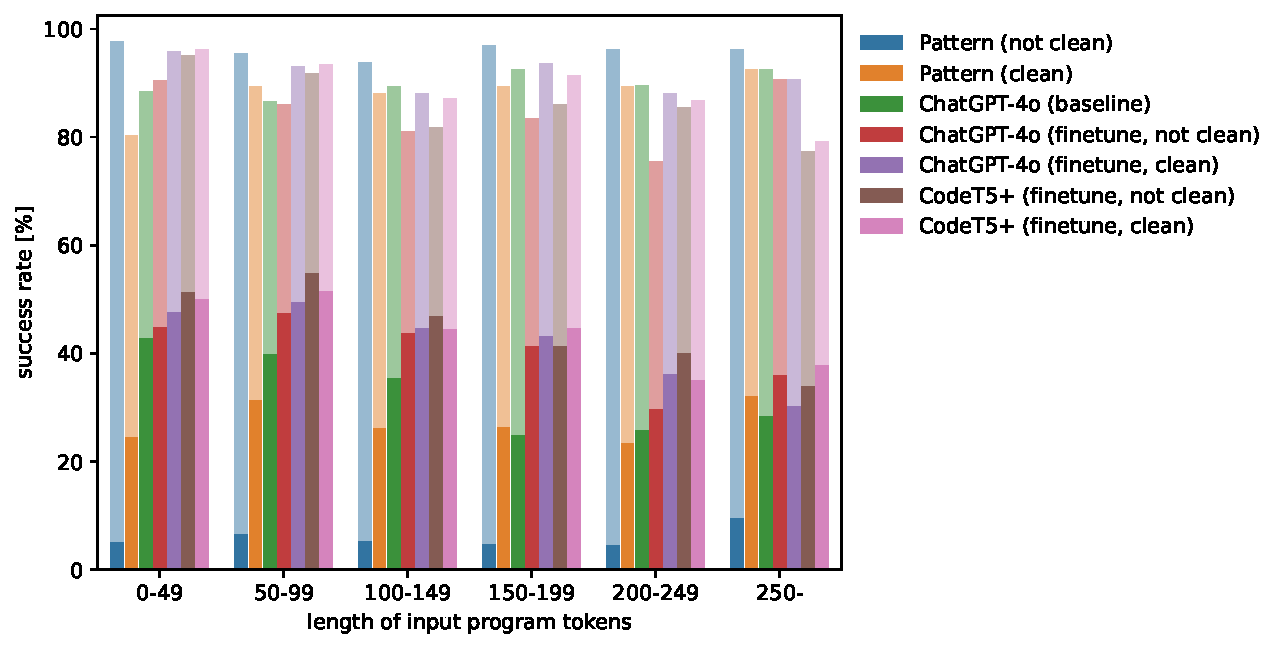
\includegraphics[width=1.0\linewidth]{Omori_fig/figure-token.pdf}
\caption{トークン別修正成功率(薄い棒グラフ:入力プログラムと等価,濃い棒グラフ:等価かつ入力プログラムより高速)}
\label{fig:eval-1:result-token}
\end{center}
\end{figure}


%%%%%%%%%%%%%%%%%%%%%%%%%%%%%%%%%%%%%%%%%%%%%%%%%%%%%%%%%%%%%%%%

%%
%% 5.3.2 考察2
%%

\subsection{修正によって短縮する実行時間}


修正によって短縮する実行時間を図\ref{fig:eval-1:result-fast-time}に示す.
深層学習モデルの中央値はいずれも1ミリ秒前後であり,モデル種別やファインチューニングの有無で実行時間は変わっていない.
ただし,ソースコードが長くなると,複数箇所を修正できる可能性があり,実行時間に与える影響は大きくなると考えられる.
また,INPが200ミリ秒を超過する場合「改善が必要」であり,マイクロベンチマーク内のプログラムが平均8.5行であることを考えると,自動リファクタリングモデルによる短縮時間は無視できない大きさであると考える.


\begin{figure}[t]
\begin{center}
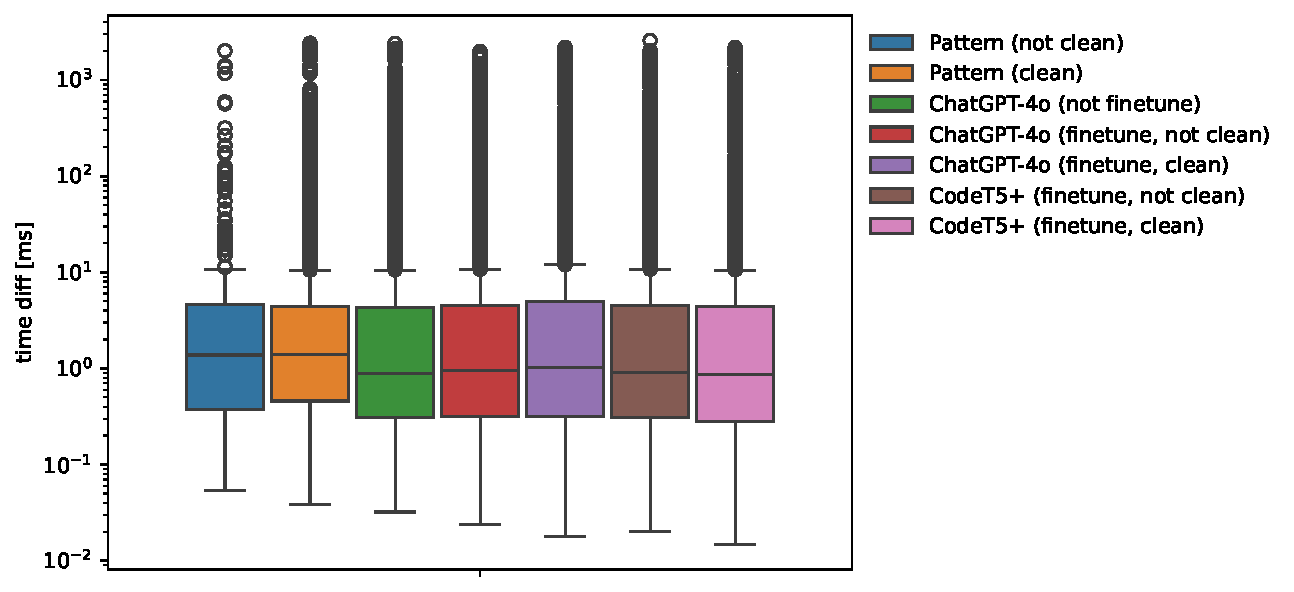
\includegraphics[width=1.0\linewidth]{Omori_fig/figure.pdf}
\caption{修正によって短縮した実行時間(入力プログラムの実行時間と生成プログラム実行時間の減算)}
\label{fig:eval-1:result-fast-time}
\end{center}
\end{figure}


%%%%%%%%%%%%%%%%%%%%%%%%%%%%%%%%%%%%%%%%%%%%%%%%%%%%%%%%%%%%%%%%

%%
%% 5.3.3 考察3
%%

\subsection{ファインチューニングすることで修正できるようになったプログラム}


ChatGPT-4oのファインチューニング前後では,ファインチューニング後に1,393件のプログラムを新たに修正できるようになった一方で,823件のプログラムの修正に失敗するようになった.

ファインチューニング前に成功していたが,ファインチューニング後に失敗するようになった入力プログラムの例をListing~\ref{result-finetune-to-failure-input}およびListing~\ref{result-finetune-to-failure-output}に示す.
\ref{result-finetune-to-failure-input}およびListing~\ref{result-finetune-to-failure-output}は,どちらもVAR\_2()関数の呼び出しを行う無名関数を非同期に実行するプログラムである.
入力プログラム(Listing~\ref{result-finetune-to-failure-input})ではsetTimeout()メソッドを用いて非同期に処理しているのに対し,ファインチューニング前のChatGPT-4oモデルはPromise.resolve()メソッドを用いて実装することで高速化している.
しかし,ファインチューニング後のChatGPT-4oモデルでは,入力プログラムと同じプログラムが出力され,修正は行われなかった.
ただし,Promiseオブジェクトが非同期処理に用いられるクラスであるのに対し,setTimeout()は本来遅延評価のための関数であるため,両関数は完全に互換があるわけではない.
実装対データセットを学習したことで,汎用性の低い修正が行われなくなったと考えられる.


\begin{figure}[t]
\captionsetup{name=Listing}
\hspace{0.04\columnwidth}
\begin{minipage}[b]{0.96\linewidth}
\begin{lstlisting}[
  caption=ファインチューニング後に失敗する例(入力),
  label=result-finetune-to-failure-input,
  captionpos=t
]
function FUNCTION_1(VAR_1) {
  setTimeout(function () {
    VAR_1("hello");
  }, 0);
}
var FUNCTION_2 = function (VAR_2) {};
FUNCTION_1(FUNCTION_2);
\end{lstlisting}
\end{minipage}

\hspace{0.04\columnwidth}
\begin{minipage}[b]{0.96\linewidth}
\begin{lstlisting}[
  caption=ファインチューニング後に失敗する例(ファインチューニング前の出力),
  label=result-finetune-to-failure-output,
  captionpos=t
]
function FUNCTION_1(VAR_1) {
  Promise.resolve().then(() => VAR_1("hello"));
}
var FUNCTION_2 = function (VAR_2) {};
FUNCTION_1(FUNCTION_2);
\end{lstlisting}
\end{minipage}
\end{figure}


また,ファインチューニング前に失敗していたが,ファインチューニング後に成功するようになった入力プログラムの例をListing~\ref{result-finetune-to-success-input}およびListing~\ref{result-finetune-to-success-output}に示す.
Listing~\ref{result-finetune-to-success-input}とListing~\ref{result-finetune-to-success-output}はどちらもJSON文字列をデシリアライズするプログラムである.
入力プログラム(Listing~\ref{result-finetune-to-success-input})ではJSON.parse()メソッドを用いてデシリアライズを行うが,ファインチューニング後のChatGPT-4oモデルの出力(Listing~\ref{result-finetune-to-success-output})ではeval()関数を用いることで実行時間を短縮している.


\begin{figure}[t]
\captionsetup{name=Listing}
\hspace{0.04\columnwidth}
\begin{minipage}[b]{0.96\linewidth}
\begin{lstlisting}[
  caption=ファインチューニング後に成功する例(入力),
  label=result-finetune-to-success-input,
  captionpos=t
]
JSON.parse('["foo","bar","baz"]');
\end{lstlisting}
\end{minipage}

\hspace{0.04\columnwidth}
\begin{minipage}[b]{0.96\linewidth}
\begin{lstlisting}[
  caption=ファインチューニング後に成功する例(ファインチューニング後の出力),
  label=result-finetune-to-success-output,
  captionpos=t
]
eval('["foo","bar","baz"]');
\end{lstlisting}
\end{minipage}
\end{figure}


さらに,ファインチューニング前後で修正に成功するが,出力が異なるプログラムの例をListing~\ref{result-finetune-both-success-input}およびListing~\ref{result-finetune-both-success-output-1},Listing~\ref{result-finetune-both-success-output-2}に示す.
各実装はいずれも配列VAR\_1内に奇数個含まれる要素を求めるプログラムである.
入力プログラム(Listing~\ref{result-finetune-both-success-input})ではfilter()メソッドを用いて2重ループを作成して同値の要素を抽出し,配列長と1のビット論理積を算出することで要素数が奇数かどうか判定している.
一方,ファインチューニング前のChatGPT-4oモデルの出力(Listing~\ref{result-finetune-both-success-output-1})では,連想配列countMapとfor文を用いて予め個数を算出し,findメソッドを用いて配列に奇数個含まれる要素を求めている.
さらにファインチューニング後のChatGPT-4oモデルの出力(Listing~\ref{result-finetune-both-success-output-2})では,ビット排他的論理和演算子を用いて簡潔に実装している.



\begin{figure}[t]
\captionsetup{name=Listing}
\hspace{0.04\columnwidth}
\begin{minipage}[b]{0.96\linewidth}
\begin{lstlisting}[
  caption=ファインチューニング前後で成功する例(入力),
  label=result-finetune-both-success-input,
  captionpos=t
]
let VAR_1 = [20, 1, -1, 2, -2, 3, 3, 5, 5, 1, 2, 4, 20, 4, -1, -2, 5];
VAR_1.filter(
  (VAR_2) => VAR_1.filter(
    (VAR_3) => VAR_3 === VAR_2
  ).length & 1
)[0];
\end{lstlisting}
\end{minipage}

\hspace{0.04\columnwidth}
\begin{minipage}[b]{0.96\linewidth}
\begin{lstlisting}[
  caption=ファインチューニング前後で成功する例(ファインチューニング前の出力),
  label=result-finetune-both-success-output-1,
  captionpos=t
]
let VAR_1 = [20, 1, -1, 2, -2, 3, 3, 5, 5, 1, 2, 4, 20, 4, -1, -2, 5];
let countMap = {};
for (let num of VAR_1) {
    countMap[num] = (countMap[num] || 0) + 1;
}
VAR_1.find(num => countMap[num] % 2 === 1);
\end{lstlisting}
\end{minipage}

\hspace{0.04\columnwidth}
\begin{minipage}[b]{0.96\linewidth}
\begin{lstlisting}[
  caption=ファインチューニング前後で成功する例(ファインチューニング後の出力),
  label=result-finetune-both-success-output-2,
  captionpos=t
]
VAR_1 = [20, 1, -1, 2, -2, 3, 3, 5, 5, 1, 2, 4, 20, 4, -1, -2, 5];
VAR_1.reduce((VAR_4, undefined) => VAR_4 ^ undefined);
\end{lstlisting}
\end{minipage}
\end{figure}


ファインチューニングによって失敗するようになる事例は成功するようになる事例よりも少ないが,無視できない数存在する.
%これは,マイクロベンチマーク内のプログラムの中に,実用的でないプログラムが混在しているためであると考える.
また,ファインチューニング前後で共通して修正できる1,357件のうち,1,324件でファインチューニングによって出力プログラムが異なることから,ファインチューニング前後のモデルを併用することが望ましいと考えられる.


%%%%%%%%%%%%%%%%%%%%%%%%%%%%%%%%%%%%%%%%%%%%%%%%%%%%%%%%%%%%%%%%

%%
%% 5.3.4 考察4
%%

\subsection{ChatGPT-4oモデルとCodeT5+モデルの比較}


図\ref{fig:eval-1:result-fast-venn3}に,ファインチューニング後のChatGPT-4oモデルとCodeT5+モデル,およびパターンマッチモデルの修正成功件数を示す.
図\ref{fig:eval-1:result-fast-venn3}より,ChatGPT-4oモデルとCodeT5+モデルで修正に成功した入力は,互いに60\%以上が共通しているものの,30\%以上は各々のモデルが固有に修正できる入力である.

Listing~\ref{result-finetune-both-success-input}およびListing~\ref{result-finetune-both-success-output-1},Listing~\ref{result-finetune-both-success-output-2}は.ファインチューニング前後のChatGPT-4oモデルがどちらも修正に成功した検証例であるが,CodeT5+モデルは入力プログラムと完全に同じプログラムを出力し,修正できなかった.
Listing~\ref{result-finetune-both-success-input}は配列処理やビット演算に加え,クロージャを用いる複雑な実装であるため,ChatGPT-4oモデルよりも事前学習データセットの規模が小さいCodeT5+モデルでは修正箇所を特定できなかったと考える.

また,ChatGPT-4oモデルで失敗し,CodeT5+モデルで成功したプログラムの例をListing~\ref{result-deep-codet5-success-input}およびListing~\ref{result-deep-codet5-success-output-1},Listing~\ref{result-deep-codet5-success-output-2}に示す.
各実装は,いずれも文字列変数VAR\_1に含まれる文字"1"を数値に変換するプログラムである.
入力プログラム(Listing~\ref{result-deep-codet5-success-input})では,正規表現を用いて"1"を抽出し,Number()コンストラクタを用いて数値に変換している.
一方,ChatGPT-4oモデルの出力(Listing~\ref{result-deep-codet5-success-output-1})では,charCodeAt()メソッドを用いて"1"をUTF-16コード単位を表す整数(49)に変換し,"0"のUTF-16コード単位を表す整数(48)を引くことで文字列"1"を数値に変換している.
また,CodeT5+モデルの出力(Listing~\ref{result-deep-codet5-success-output-2})では,slice()メソッドを用いて"1"を抽出し,parseInt()関数を用いて文字列を数値に変換している.
ChatGPT-4oモデルの出力(Listing~\ref{result-deep-codet5-success-output-1})も,入力プログラムと機能的には等価であるが,文字列をUTF-16コード単位を表す整数に変換していることから,高速化には失敗している.


\begin{figure}[t]
\captionsetup{name=Listing}
\hspace{0.04\columnwidth}
\begin{minipage}[b]{0.96\linewidth}
\begin{lstlisting}[
  caption=ChatGPT-4oで失敗し,CodeT5+で成功した例(入力),
  label=result-deep-codet5-success-input,
  captionpos=t
]
var VAR_1 = "(1)";
Number(VAR_1.match(/\d/));
\end{lstlisting}
\end{minipage}

\hspace{0.04\columnwidth}
\begin{minipage}[b]{0.96\linewidth}
\begin{lstlisting}[
  caption=ChatGPT-4oで失敗し,CodeT5+で成功した例(ChatGPT-4oの出力),
  label=result-deep-codet5-success-output-1,
  captionpos=t
]
var VAR_1 = "(1)";
VAR_1.charCodeAt(1) - 48;
\end{lstlisting}
\end{minipage}

\hspace{0.04\columnwidth}
\begin{minipage}[b]{0.96\linewidth}
\begin{lstlisting}[
  caption=ChatGPT-4oで失敗し,CodeT5+で成功した例(CodeT5+の出力),
  label=result-deep-codet5-success-output-2,
  captionpos=t
]
var VAR_1 = "(1)";
parseInt(VAR_1.slice(1));
\end{lstlisting}
\end{minipage}
\end{figure}


ChatGPT-4oとCodeT5+の両モデルで修正に成功するが,出力が異なるプログラムをListing~\ref{result-deep-both-success-input}およびListing~\ref{result-deep-both-success-output-1},Listing~\ref{result-deep-both-success-output-2}に示す.
各実装は,いずれも文字列"in Downtown Brooklyn"から最初の空白文字より後の文字列を抽出するプログラムである.
入力プログラム(Listing~\ref{result-deep-both-success-input})では,正規表現を用いて文字列を空白文字で分割し,filter()メソッドを用いて分割した最初の文字列("in")を除外し,join()メソッドを用いて残りの文字列を再び空白文字で結合している.
一方で,ChatGPT-4oモデルの出力(Listing~\ref{result-deep-both-success-output-1})では,indexOf()メソッドを用いて最も文頭に近い空白文字の位置を求め,substr()メソッドを用いて空白文字より後の文字列を抽出している.
また,CodeT5+モデルの出力(Listing~\ref{result-deep-both-success-output-2})では,正規表現を用いずに文字列を空白文字で分割し,filter()メソッドの代わりにslice()メソッドを用いて2番目以降の要素を抽出し,join()メソッドを用いて残りの文字列を再び空白文字で結合している.



\begin{figure}[t]
\captionsetup{name=Listing}
\hspace{0.04\columnwidth}
\begin{minipage}[b]{0.96\linewidth}
\begin{lstlisting}[
  caption=ChatGPT-4oとCodeT5+の両モデルで修正に成功する例(入力),
  label=result-deep-both-success-input,
  captionpos=t
]
var VAR_1 = "in Downtown Brooklyn";
var VAR_2 = VAR_1
  .split(/\s+/)
  .filter((VAR_3, VAR_4) => VAR_4 !== 0)
  .join(" ");
\end{lstlisting}
\end{minipage}

\hspace{0.04\columnwidth}
\begin{minipage}[b]{0.96\linewidth}
\begin{lstlisting}[
  caption=ChatGPT-4oとCodeT5+の両モデルで成功する例(ChatGPT-4oの出力),
  label=result-deep-both-success-output-1,
  captionpos=t
]
var VAR_1 = "in Downtown Brooklyn";
var VAR_2 = VAR_1.substr(VAR_1.indexOf(" ") + 1);
\end{lstlisting}
\end{minipage}

\hspace{0.04\columnwidth}
\begin{minipage}[b]{0.96\linewidth}
\begin{lstlisting}[
  caption=ChatGPT-4oとCodeT5+の両モデルで成功する例(CodeT5+の出力),
  label=result-deep-both-success-output-2,
  captionpos=t
]
var VAR_1 = "in Downtown Brooklyn";
var VAR_2 = VAR_1.split(" ").slice(1).join(" ");
\end{lstlisting}
\end{minipage}
\end{figure}


\todo{}
表\ref{table:eval-1:result-test-fast}から,CodeT5+モデルの方が修正成功件数はやや多いが,大きく上回っているわけではない.
ChatGPT-4oとCodeT5+の各モデルのみで修正できる事例は無視できない数存在することから,前節同様,2種のモデルを併用することが望ましいと考えられる.


\begin{figure}[t]
\begin{center}
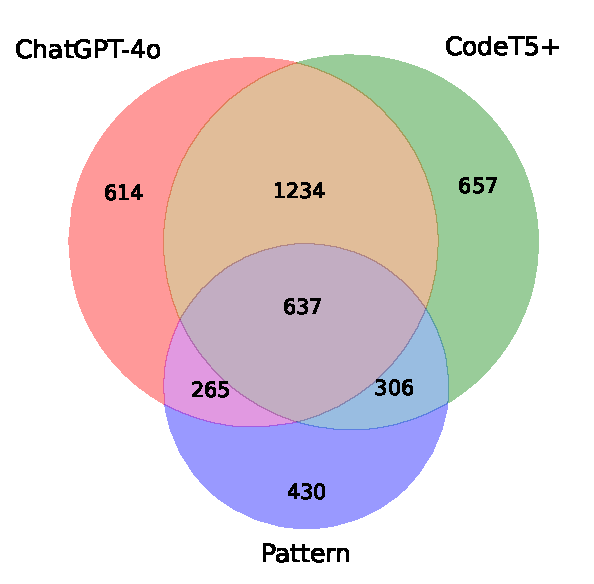
\includegraphics[width=0.5\linewidth]{Omori_fig/figure-venn3.pdf}
\caption{result}
\label{fig:eval-1:result-fast-venn3}
\end{center}
\end{figure}


%%%%%%%%%%%%%%%%%%%%%%%%%%%%%%%%%%%%%%%%%%%%%%%%%%%%%%%%%%%%%%%%

%%
%% 5.3.5 考察5
%%

\subsection{深層学習モデルとパターンマッチモデルの差異}


Listing~\ref{result-deep-both-success-input}およびListing~\ref{result-deep-both-success-output-1},Listing~\ref{result-deep-both-success-output-2}は.ChatGPT-4oモデルおよびCodeT5+モデルがどちらも修正に成功した検証例であるが,パターンマッチモデルでは修正できなかった.
Listing~\ref{result-deep-both-success-input}は複数のメソッドを用いており,マッチするパターンが多くなった結果,組み合わせが膨大になり,修正できなかったと考える.

一方,パターンマッチモデルでは成功したが,深層学習モデルでは修正できなかった例も存在する.
パターンマッチモデルのみ修正に成功した例をListing~\ref{result-pattern-deep-success-input}およびListing~\ref{result-pattern-deep-success-output}に示す.
各実装は,どちらも適当な数値の小数点以下を切り捨てる関数FUNCTION\_1を実装するプログラムである.
入力プログラム(Listing~\ref{result-pattern-deep-success-input})はMath.floor()メソッドを用いて小数点以下切り捨てによる数値の丸め処理を行う.
また,パターンマッチモデルの出力(Listing~\ref{result-pattern-deep-success-output})は,ビット否定演算子を用いて小数点以下切り捨てによる数値の丸め処理を行う.
通常の数値は64ビットであるのに対してビット否定の演算結果は32ビットに変換されるため,一度ビット否定を算出し,もう一度ビット否定を算出することで小数点以下を切り捨てることができる.



\begin{figure}[t]
\captionsetup{name=Listing}
\hspace{0.04\columnwidth}
\begin{minipage}[b]{0.96\linewidth}
\begin{lstlisting}[
  caption=パターンマッチモデルでのみ成功する例(入力),
  label=result-pattern-deep-success-input,
  captionpos=t
]
function FUNCTION_1(VAR_1, VAR_2) {
  return Math.floor(Math.random() * (VAR_2 - VAR_1 + 1) + VAR_1);
}
FUNCTION_1(1, 6);
\end{lstlisting}
\end{minipage}

\hspace{0.04\columnwidth}
\begin{minipage}[b]{0.96\linewidth}
\begin{lstlisting}[
  caption=パターンマッチモデルでのみ成功する例(パターンマッチの出力),
  label=result-pattern-deep-success-output,
  captionpos=t
]
function FUNCTION_1(VAR_1, VAR_2) {
  return ~~(Math.random() * (VAR_2 - VAR_1 + 1) + VAR_1);
}
FUNCTION_1(1, 6);
\end{lstlisting}
\end{minipage}
\end{figure}


上記の例のように,深層学習,パターンマッチの各モデルのみで修正できる事例は一定数存在することから,モデルを併用することで,より多くのプログラムを高速化できると考えられる.
ただし,本実験では深層学習モデルが1件の入力に1件の修正プログラムを出力するのに対し,パターンマッチモデルが最大10件の修正プログラムを出力することに留意を要する.
等価性の検証や実行時間の比較にも時間がかかることから,修正成功率が比較的低いパターンマッチモデルは,時間対効果の観点から深層学習モデルに比べて自動リファクタリングモデルとして有用でないと考える.


\begin{comment}


%%%%%%%%%%%%%%%%%%%%%%%%%%%%%%%%%%%%%%%%%%%%%%%%%%%%%%%%%%%%%%%%

%%
%% 6 GitHub Pull Requestに対する修正性能評価
%%

\chapter{GitHub Pull Requestに対する修正性能評価}\label{chapter:eval-2}


%%%%%%%%%%%%%%%%%%%%%%%%%%%%%%%%%%%%%%%%%%%%%%%%%%%%%%%%%%%%%%%%

%%
%% 6.1 実験方法
%%

\section{実験方法}


本章では,GitHub Pull Requestを用いて提案モデルと既存モデルの修正性能を比較する.
\todo{それによって何を明らかにしようとしている?}
%実装対の内,より低速な実装に対して各モデルが修正したプログラムの高速化性能を分析する.


\begin{figure}[t]
\centerline{
\includegraphics[width=0.8\linewidth]{Omori_fig/dummy.pdf}}
\caption{overview}
\label{fig-dummy}
\end{figure}


%%%%%%%%%%%%%%%%%%%%%%%%%%%%%%%%%%%%%%%%%%%%%%%%%%%%%%%%%%%%%%%%

%%
%% 6.1.1 評価データセット
%%

\subsection{評価データセット}


npm.js\footnote{\url{https://www.npmjs.com/}}からキーワードに「server」または「backend」を含むプロジェクトを収集する.
本研究では,サーバサイドのプログラムの方が多くのクエリに対処を要するため,複合的な実行時間の低下が考えられる.

収集したプロジェクトのGitHubリポジトリから高速化のためのリファクタリングを抽出する.
そして,タイトルまたは説明文に\todo{}のいずれかの単語を含むPull Requestを収集する.
さらに,Pull Requestの前後でプログラムのテストを実行したときに,どちらも成功して,かつ実行時間が短くなったもの

結果として,\todo{}件のGitHub Pull Requestを対象に提案モデルの修正性能を調査する.
%% 771 PR, 128 Prj, 


%%%%%%%%%%%%%%%%%%%%%%%%%%%%%%%%%%%%%%%%%%%%%%%%%%%%%%%%%%%%%%%%

%%
%% 6.1.2 評価対象モデル
%%

\subsection{評価対象モデル}
本章では,提案モデルの中でも\ref{chapter:eval-1}章で性能が高かった,データクレンジング済み実装対データセットを学習したモデルの性能を調査する.
また,ベースラインとしてファインチューニングを行っていないChatGPT-4oモデル,および開発者の修正と修正性能を比較する.

したがって,本章では表~\ref{table:eval-2:models}に示す5件のモデルと開発者の修正の6通りのプログラムの修正性能を比較する.


\begin{table}[t]
\caption{評価対象モデル}
\label{table:eval-2:models}
\centering
\begin{tabular}{lc}
\hline
モデル & ファインチューニング\\
\hline
パターンマッチ & - \\
CodeT5+ & あり \\
CodeT5+ & なし \\
ChatGPT-4o & あり \\
ChatGPT-4o & なし \\
\hline
\end{tabular}
\end{table}


%%%%%%%%%%%%%%%%%%%%%%%%%%%%%%%%%%%%%%%%%%%%%%%%%%%%%%%%%%%%%%%%

%%
%% 6.2 結果
%%

\section{結果}


%%%%%%%%%%%%%%%%%%%%%%%%%%%%%%%%%%%%%%%%%%%%%%%%%%%%%%%%%%%%%%%%

%%
%% 6.3 考察
%%

\section{考察}


\end{comment}


%%%%%%%%%%%%%%%%%%%%%%%%%%%%%%%%%%%%%%%%%%%%%%%%%%%%%%%%%%%%%%%%

%%
%% 7 妥当性への脅威
%%

\chapter{妥当性への脅威}\label{chapter:threats}


%%%%%%%%%%%%%%%%%%%%%%%%%%%%%%%%%%%%%%%%%%%%%%%%%%%%%%%%%%%%%%%%

%%
%% 7.1 内的妥当性
%%

\section{内的妥当性}


本研究では,データセットの前処理に抽象構文木を用いる.
その際,文章量の多いプログラムを抽象構文木に変換するために長時間かかるため,文字数が多い上位5\%のプログラムを除外し,95\%分位までのプログラムのみを対象とした.
その結果,データセットはマイクロベンチマーク共有サービス上のプログラムを網羅できておらず,評価実験結果に影響を与える恐れがある.
ただし,非常に長いプログラムの修正は現在の大規模言語モデルにとって困難なタスクであり,本研究でもCodeT5+の入出力最大長は512トークンに制限している.
そのため,本研究の目的であるマイクロベンチマーク共有サービス上のプログラムを学習した大規模言語モデルの修正性能を明らかにする上での影響は小さいと考える.

本研究では,マイクロベンチマーク共有サービスJsPerfからプログラムを収集している.
当該サービスは2020年にサービスを終了しているため,データセットには2020年7月までのプログラムしか含まれない.
したがって,検証結果が現在でも高速な実装方法であるとは限らない.
本研究では,収集データセットの中で,最新リビジョン(JsPerfには既存のマイクロベンチマークを修正し,新たなリビジョンとして保存する機能が有る)のプログラムセットのみをデータセットに使用することで,データセット内での古い実装方法の比重を抑えるように可能な限り努めた.
より正確な結果を得るためには他のマイクロベンチマーク共有サービスから継続的にプログラムを収集する必要がある.

本研究ではJavaScriptを実行する際に,サーバサイドJavaScript動作環境であるNodeJSを使用している.
NodeJSはJavaScriptエンジンとしてV8\footnote{\url{https://v8.dev/}}を採用しており,V8はGoogle ChromeやMicrosoft EdgeをはじめとするChromiumベースのブラウザアプリケーションでも広く用いられている.
一方で,SpiderMonkey\footnote{\url{https://spidermonkey.dev/}}やJavaScriptCore\footnote{\url{https://developer.apple.com/documentation/javascriptcore/}}等のJavaScriptエンジンを採用するJavaScript実行環境も存在する.
JavaScriptエンジンが異なる環境ではJITコンパイルアルゴリズムも異なるため,本研究で作成した実装対が一般にV8以外のJavaScriptエンジンでも効果的なリファクタリングであるとは限らない.
本研究の評価実験結果はV8エンジンに限定した結果であるが,方法論については他のJavaScriptエンジンについても同様の手順で進行できるものであると考える.

\todo{データクレンジングについて,削除が結果に与える影響・今後データは増やせそうか}


%%%%%%%%%%%%%%%%%%%%%%%%%%%%%%%%%%%%%%%%%%%%%%%%%%%%%%%%%%%%%%%%

%%
%% 7.2 外的妥当性
%%

\section{外的妥当性}


本研究では,マイクロベンチマーク共有サービス上のプログラムを対象に深層学習モデルのリファクタリング性能を明らかにしたが,多くのマイクロベンチマークプログラムは非常に短く,演算結果の代入や出力が省略されていることが多い.
また,効果的に実行速度の差を測定するために巨大な配列や長大なループが用いられている.
そのため,ライブラリのように実用目的で十分に保守されたソフトウェアとはプログラムの実装方法やリファクタリング時の影響が異なると考えられる.


%%%%%%%%%%%%%%%%%%%%%%%%%%%%%%%%%%%%%%%%%%%%%%%%%%%%%%%%%%%%%%%%

%%
%% 8 おわりに
%%

\chapter{おわりに}\label{chapter:conc}


本研究では,高速化のための自動リファクタリングモデルの作成に利用できる39,009件の実装対データセットを作成したとともに,作成した実装対データセットを学習させた自動リファクタリングモデルの高速化性能を調査した.


調査の結果,マイクロベンチマーク共有サービス上のプログラムに対しては,本研究で作成したモデルが既存の大規模言語モデルより11.0ポイント多いプログラムに対して高速化リファクタリングに成功した.
\todo{}


%%%%%%%%%%%%%%%%%%%%%%%%%%%%%%%%%%%%%%%%%%%%%%%%%%%%%%%%%%%%%%%%

%%
%% 謝辞
%%

%\begin{acknowledgements}
%感謝します.
%\end{acknowledgements}


%%%%%%%%%%%%%%%%%%%%%%%%%%%%%%%%%%%%%%%%%%%%%%%%%%%%%%%%%%%%%%%%

%%
%% 参考文献
%%

\begin{thebibliography}{99}


\bibitem{Falleri_2014}
    J. R. Falleri, F. Morandat, X. Blanc, M. Martinez, and M. Monperrus,
    "Fine-grained and accurate source code differencing,"
    in Proceedings of the 29th ACM/IEEE International Conference on Automated Software Engineering (ASE),
    2014,
    pp.313-324.

\bibitem{Gong_2015}
    L. Gong, M. Pradel, and K. Sen,
    "JITProf: pinpointing JIT-unfriendly JavaScript code,"
    in Proceedings of the 2015 10th Joint Meeting on Foundations of Software Engineering (ESEC/FSE),
    2015,
    pp.357-368.

\bibitem{Selakovic_2016}
    M. Selakovic, and M. Pradel,
    "Performance issues and optimizations in JavaScript: an empirical study,"
    in Proceedings of the 38th International Conference on Software Engineering (ICSE),
    2016,
    pp.61-72.

\bibitem{Selakovic_2017}
    M. Selakovic, T. Glaser, and M. Pradel,
    "An actionable performance profiler for optimizing the order of evaluations,"
    in Proceedings of the 26th ACM SIGSOFT International Symposium on Software Testing and Analysis (ISSTA),
    2017,
    pp.170-180.

\bibitem{Saiki_2021}
    K. Saiki, and A. Ihara,
    "Linkage of Similar Code Snippets Assessed in the Micro Benchmark Service jsPerf,"
    in Proceedings of the 21th IEEE International Working Conference on Source Code Analysis and Manipulation (SCAM),
    2021,
    pp.247-251.

\bibitem{Shirafuji_2023}
    A. Shirafuji, Y. Oda, J, Suzuki, M. Morishita, and Y. Watanobe,
    "Refactoring Programs Using Large Language Models with Few-shot Examples,"
    in Proceedings of the 30th Asia-Pacific Software Engineering Conference (APSEC),
    2023,
    pp.151-160.

\bibitem{Wang_2023}
    Y. Wang, H. Le, A. D. Gotmare, N. D. Q. Bui, J. Li, and S. C. H. Hoi,
    "CodeT5+: Open Code Large Language Models for Code Understanding and Generation,"
    arXiv preprint,
    2023.

\bibitem{Ishizue_2024}
    R. Ishizue, K. Sakamoto, H. Washizaki, and Y. Fukazawa,
    "Improved Program Repair Methods using Refactoring with GPT Models,"
    in Proceedings of the 55th ACM Technical Symposium on Computer Science Education (SIGCSE),
    2024,
    pp.569-575.


\end{thebibliography}


%%%%%%%%%%%%%%%%%%%%%%%%%%%%%%%%%%%%%%%%%%%%%%%%%%%%%%%%%%%%%%%%

%%
%% 付録
%%

% \appendix
% 
% \chapter{サンプルプログラム}
% 
% プログラムリストや実行結果など,本論を補足する上で必要と思われるものが
% あれば付録として付ける.
% 
% {
% \footnotesize
% \begin{verbatim}
% #include <stdio.h>
% int main(void)
% {
%     printf("Hello, World!\n");
%     return 0;
% }
% \end{verbatim}
% }


%%%%%%%%%%%%%%%%%%%%%%%%%%%%%%%%%%%%%%%%%%%%%%%%%%%%%%%%%%%%%%%%

\end{document}
